% Soubory musí být v kódování, které je nastaveno v příkazu \usepackage[...]{inputenc}

\documentclass[%        Základní nastavení
%  draft,    				  % Testovací překlad
  12pt,       				% Velikost základního písma je 12 bodů
  a4paper,    				% Formát papíru je A4
  oneside,      			% Jednostranný tisk
	%twoside,      			% Dvoustranný tisk (kapitoly a další důležité části tedy začínají na lichých stranách)
	unicode,						% Záložky a metainformace ve výsledném  PDF budou v kódování unicode
]{report}				    	% Dokument třídy 'zpráva', vhodná pro sazbu závěrečných prací s kapitolami

\usepackage[utf8]		  %	Kódování zdrojových souborů je UTF-8
	{inputenc}					% Balíček pro nastavení kódování zdrojových souborů

\usepackage[				% Nastavení geometrie stránky
	bindingoffset=10mm,		% Hřbet pro vazbu
	hmargin={25mm,25mm},	% Vnitřní a vnější okraj
	vmargin={25mm,34mm},	% Horní a dolní okraj
	footskip=17mm,			  % Velikost zápatí
	nohead,					      % Bez záhlaví
	marginparsep=2mm,		  % Vzdálenost marginálií
	marginparwidth=18mm,	% Šířka marginálií
]{geometry}

\usepackage{sectsty}
	%přetypuje nadpisy všech úrovní na bezpatkové, kromě \chapter, která je přenastavena zvlášť v thesis.sty
	\allsectionsfont{\sffamily}

\usepackage{graphicx} % Balíček 'graphicx' pro vkládání obrázků
											% Nutné pro vložení logotypů školy a fakulty

\usepackage[          % Balíček 'acronym' pro sazby zkratek a symbolů
	nohyperlinks				% Nebudou tvořeny hypertextové odkazy do seznamu zkratek
]{acronym}						
											% Nutné pro použití prostředí 'acronym' balíčku 'thesis'

\usepackage[
	breaklinks=true,		% Hypertextové odkazy mohou obsahovat zalomení řádku
	hypertexnames=false % Názvy hypertext. odkazů budou tvořeny nezávisle na názvech TeXu
]{hyperref}						% Balíček 'hyperref' pro sazbu hypertextových odkazů
											% Nutné pro použití příkazu 'pdfsettings' balíčku 'thesis'

\usepackage{pdfpages} % Balíček umožňující vkládat stránky z PDF souborů
                      % Nutné při vkládání titulních listů a zadání přímo
                      % ve formátu PDF z informačního systému

\usepackage{enumitem} % Balíček pro nastavení mezerování v odrážkách
  \setlist{topsep=0pt,partopsep=0pt,noitemsep} % konkrétní nastavení

\usepackage{cmap} 		% Balíček cmap zajišťuje, že PDF vytvořené `pdflatexem' je
											% plně "prohledávatelné" a "kopírovatelné"

%\usepackage{upgreek}	% Balíček pro sazbu stojatých řeckých písmem
											%% např. stojaté pí: \uppi
											%% např. stojaté mí: \upmu (použitelné třeba v mikrometrech)
											%% pozor, grafická nekompatibilita s fonty typu Computer Modern!
                      
%\usepackage{amsmath} %balíček pro sabu náročnější matematiky                 

\usepackage{dirtree}	% sazba adresářové struktury
                      % vhodné pro prezentaci obsahu elektronické přílohy (např. CD)

\usepackage{multicol}
\usepackage{array,multirow}
\usepackage{rotating}
\usepackage{xcolor,colortbl}
\usepackage{amsmath}

\definecolor{ForestGreen}{RGB}{34,139,34}
\definecolor{light-gray}{gray}{0.95}




\usepackage[formats]{listings}	% Balíček pro sazbu zdrojových textů
\lstset{              % nastavení
%	Definice jazyka použitého ve výpisech
%    language=[LaTeX]{TeX},	% LaTeX
%	language={Matlab},		% Matlab
	language={C},           % jazyk C
    basicstyle=\fontsize{10}{14}\selectfont\ttfamily,
    tabsize=2,			% definice velikosti tabulátoru
    showstringspaces=false,
    numbers=left,                    
    commentstyle=\color{ForestGreen},
    keywordstyle=\color{blue},
    stringstyle=\color{olive},
    backgroundcolor=\color{light-gray},
    inputencoding=utf8,         % pro soubory uložené v kódování UTF-8
		columns=fixed,  %fixed nebo flexible,
		fontadjust=true %licovani sloupcu
    extendedchars=true,
    literate=%  definice symbolů s diakritikou
    {á}{{\'a}}1
    {č}{{\v{c}}}1
    {ď}{{\v{d}}}1
    {é}{{\'e}}1
    {ě}{{\v{e}}}1
    {í}{{\'i}}1
    {ň}{{\v{n}}}1
    {ó}{{\'o}}1
    {ř}{{\v{r}}}1
    {š}{{\v{s}}}1
    {ť}{{\v{t}}}1
    {ú}{{\'u}}1
    {ů}{{\r{u}}}1
    {ý}{{\'y}}1
    {ž}{{\v{z}}}1
    {Á}{{\'A}}1
    {Č}{{\v{C}}}1
    {Ď}{{\v{D}}}1
    {É}{{\'E}}1
    {Ě}{{\v{E}}}1
    {Í}{{\'I}}1
    {Ň}{{\v{N}}}1
    {Ó}{{\'O}}1
    {Ř}{{\v{R}}}1
    {Š}{{\v{S}}}1
    {Ť}{{\v{T}}}1
    {Ú}{{\'U}}1
    {Ů}{{\r{U}}}1
    {Ý}{{\'Y}}1
    {Ž}{{\v{Z}}}1
}

%%%%%%%%%%%%%%%%%%%%%%%%%%%%%%%%%%%%%%%%%%%%%%%%%%%%%%%%%%%%%%%%%
%%%%%%      Definice informací o dokumentu             %%%%%%%%%%
%%%%%%%%%%%%%%%%%%%%%%%%%%%%%%%%%%%%%%%%%%%%%%%%%%%%%%%%%%%%%%%%%

% V tomto souboru se nastavují téměř veškeré informace, proměnné mezi studenty:
% jméno, název práce, pohlaví atd.
% Tento soubor je SDÍLENÝ mezi textem práce a prezentací k obhajobě -- netřeba něco nastavovat na dvou místech.

\usepackage[
%%% Z následujících voleb jazyka lze použít pouze jednu
  czech-english,		% originální jazyk je čeština, překlad je anglicky (výchozí)
  %english-czech,	% originální jazyk je angličtina, překlad je česky
  %slovak-english,	% originální jazyk je slovenština, překlad je anglicky
  %english-slovak,	% originální jazyk je angličtina, překlad je slovensky
%
%%% Z následujících voleb typu práce lze použít pouze jednu
  %semestral,		  % semestrální práce (nesází se abstrakty, prohlášení, poděkování) (výchozí)
  %bachelor,			%	bakalářská práce
  master,			  % diplomová práce
  %treatise,			% pojednání o disertační práci
  %doctoral,			% disertační práce
%
%%% Z následujících voleb zarovnání objektů lze použít pouze jednu
%  left,				  % rovnice a popisky plovoucích objektů budou zarovnány vlevo
	center,			    % rovnice a popisky plovoucích objektů budou zarovnány na střed (vychozi)
%
]{thesis}   % Balíček pro sazbu studentských prací


%%% Jméno a příjmení autora ve tvaru
%  [tituly před jménem]{Křestní}{Příjmení}[tituly za jménem]
% Pokud osoba nemá titul před/za jménem, smažte celý řetězec '[...]'
\author[Bc.]{David}{Lindtner}

%%% Identifikační číslo autora (VUT ID)
\butid{196815}

%%% Pohlaví autora/autorky
% (nepoužije se ve variantě english-czech ani english-slovak)
% Číselná hodnota: 1...žena, 0...muž
\gender{0}

%%% Jméno a příjmení vedoucího/školitele včetně titulů
%  [tituly před jménem]{Křestní}{Příjmení}[tituly za jménem]
% Pokud osoba nemá titul před/za jménem, smažte celý řetězec '[...]'
\advisor[Ing.]{Petr}{Gábrlík}[Ph.D.]

%%% Jméno a příjmení oponenta včetně titulů
%  [tituly před jménem]{Křestní}{Příjmení}[tituly za jménem]
% Pokud osoba nemá titul před/za jménem, smažte celý řetězec '[...]'
% Nastavení oponenta se uplatní pouze v prezentaci k obhajobě;
% v případě, že nechcete, aby se na titulním snímku prezentace zobrazoval oponent, pouze příkaz zakomentujte;
% u obhajoby semestrální práce se oponent nezobrazuje (jelikož neexistuje)
% U dizertační práce jsou typicky dva až tři oponenti. Pokud je chcete mít na titulním slajdu, prosím ručně odkomentujte a upravte jejich jména v definici "VUT title page" v souboru thesis.sty.
\opponent[doc.\ Mgr.]{Křestní}{Příjmení}[Ph.D.]

%%% Název práce
%  Parametr ve složených závorkách {} je název v originálním jazyce,
%  parametr v hranatých závorkách [] je překlad (podle toho jaký je originální jazyk).
%  V případě, že název Vaší práce je dlouhý a nevleze se celý do zápatí prezentace, použijte příkaz
%  \def\insertshorttitle{Zkác.\ náz.\ práce}
%  kde jako parametr vyplníte zkrácený název. Pokud nechcete zkracovat název, budete muset předefinovat,
%  jak se vytváří patička slidu. Viz odkaz: https://bit.ly/3EJTp5A
\title[Simulation of Unmanned Aircrafts in a Virtual Environment]{Simulace bezpilotních letadel ve virtuálním prostředí}

%%% Označení oboru studia
%  Parametr ve složených závorkách {} je název oboru v originálním jazyce,
%  parametr v hranatých závorkách [] je překlad
\specialization[Cybernetics, Control and Measurements]{Kybernetika, automatizace a měření}

%%% Označení ústavu
%  Parametr ve složených závorkách {} je název ústavu v originálním jazyce,
%  parametr v hranatých závorkách [] je překlad
\department[Department of Control and Instrumentation]{Ústav automatizace a měřicí techniky}
%\department[Department of Biomedical Engineering]{Ústav biomedicínského inženýrství}
%\department[Department of Electrical Power Engineering]{Ústav elektroenergetiky}
%\department[Department of Electrical and Electronic Technology]{Ústav elektrotechnologie}
%\department[Department of Physics]{Ústav fyziky}
%\department[Department of Foreign Languages]{Ústav jazyků}
%\department[Department of Mathematics]{Ústav matematiky}
%\department[Department of Microelectronics]{Ústav mikroelektroniky}
%\department[Department of Radio Electronics]{Ústav radioelektroniky}
%\department[Department of Theoretical and Experimental Electrical Engineering]{Ústav teoretické a experimentální elektrotechniky}
%\department[Department of Telecommunications]{Ústav telekomunikací}
%\department[Department of Power Electrical and Electronic Engineering]{Ústav výkonové elektrotechniky a elektroniky}

%%% Označení fakulty
%  Parametr ve složených závorkách {} je název fakulty v originálním jazyce,
%  parametr v hranatých závorkách [] je překlad
%\faculty[Faculty of Architecture]{Fakulta architektury}
\faculty[Faculty of Electrical Engineering and~Communication]{Fakulta elektrotechniky a~komunikačních technologií}
%\faculty[Faculty of Chemistry]{Fakulta chemická}
%\faculty[Faculty of Information Technology]{Fakulta informačních technologií}
%\faculty[Faculty of Business and Management]{Fakulta podnikatelská}
%\faculty[Faculty of Civil Engineering]{Fakulta stavební}
%\faculty[Faculty of Mechanical Engineering]{Fakulta strojního inženýrství}
%\faculty[Faculty of Fine Arts]{Fakulta výtvarných umění}
%
%Nastavení logotypu (v hranatych zavorkach zkracene logo, ve slozenych plne):
\facultylogo[logo/FEKT_zkratka_barevne_PANTONE_CZ]{logo/UTKO_color_PANTONE_CZ}

%%% Rok odevzdání práce
\graduateyear{2022}
%%% Akademický rok odevzdání práce
\academicyear{2021/22}

%%% Datum obhajoby (uplatní se pouze v prezentaci k obhajobě)
\date{11.\,11.\,1980} 

%%% Místo obhajoby
% Na titulních stránkách bude automaticky vysázeno VELKÝMI písmeny (pokud tyto stránky sází šablona)
\city{Brno}

%%% Abstrakt
\abstract
[The master thesis deals with the issue of simulation of unmanned aircraft missions in~a~virtual environment. The aim of the work is to demonstrate basic and more advanced autonomous aerial missions in the simulated environment Gazebo - ROS 2. The work emphasizes the stability of the software solution and the stability of the communication between critical components of the aerial mission.
]{%
Diplomová práce se zabývá problematikou simulace misí bezpilotních letadel ve virtuálním prostředí. Cílem práce je demonstrovat základní i pokročilejší autonomní letecké mise v~simulovaném prostředí Gazebo - ROS 2. Důraz práce je kladen na stabilitu softwarového řešení a stabilitu komunikace mezi kritickými komponenty letecké mise.
}

%%% Klíčová slova
\keywrds[%
Autonomous mission, Robotics, Drone, Pixhawk, PX4, Autopilot uORB, DDS, RTPS, MAVlink, Mavros, ROS 2, Gazebo, Simulation
]{%
Autonomní mise, Robotika, Dron, Pixhawk, PX4, Autopilot, uORB, DDS, RTPS, MAVLink, Mavros ROS 2, Gazebo, Simulace
}

%%% Poděkování
\acknowledgement{%
Rád bych poděkoval vedoucímu diplomové práce panu Ing.~Petrovi Gabrlíkovi, Ph.D.\ za~odborné vedení, trpělivost, čas strávený na konzultacích a podnětné návrhy k~práci. Dále bych rád poděkoval Bc. Milošovi Cihlářovi za~poskytnutí dat k sestavení simulačního modelu okolí naší školy, které byli výsledkem jeho diplomové práce.
}%
  % do tohoto souboru doplňte údaje o sobě, druhu práce, názvu...

%%%%%%%%%%%%%%%%%%%%%%%%%%%%%%%%%%%%%%%%%%%%%%%%%%%%%%%%%%%%%%%%%%%%%%%%

%%%%%%%%%%%%%%%%%%%%%%%%%%%%%%%%%%%%%%%%%%%%%%%%%%%%%%%%%%%%%%%%%%%%%%%%
%%%%%%     Nastavení polí ve Vlastnostech dokumentu PDF      %%%%%%%%%%%
%%%%%%%%%%%%%%%%%%%%%%%%%%%%%%%%%%%%%%%%%%%%%%%%%%%%%%%%%%%%%%%%%%%%%%%%
%% Při načteném balíčku 'hyperref' lze použít příkaz '\pdfsettings':
\pdfsettings
%  Nastavení polí je možné provést také ručně příkazem:
%\hypersetup{
%  pdftitle={Název studentské práce},    	% Pole 'Document Title'
%  pdfauthor={Autor studenstké práce},   	% Pole 'Author'
%  pdfsubject={Typ práce}, 						  	% Pole 'Subject'
%  pdfkeywords={Klíčová slova}           	% Pole 'Keywords'
%}
%%%%%%%%%%%%%%%%%%%%%%%%%%%%%%%%%%%%%%%%%%%%%%%%%%%%%%%%%%%%%%%%%%%%%%%

\pdfmapfile{=vafle.map}

%%%%%%%%%%%%%%%%%%%%%%%%%%%%%%%%%%%%%%%%%%%%%%%%%%%%%%%%%%%%%%%%%%%%%%%
%%%%%%%%%%%       Začátek dokumentu               %%%%%%%%%%%%%%%%%%%%%
%%%%%%%%%%%%%%%%%%%%%%%%%%%%%%%%%%%%%%%%%%%%%%%%%%%%%%%%%%%%%%%%%%%%%%%
\begin{document}
\pagestyle{empty} %vypnutí číslování stránek

%%% Vložení desek -- od září 2021 na žádost fakulty nepoužíváno
%\includepdf[pages=1]%  buďto generovaných informačním systémem
  %{pdf/student-desky}% název souboru nesmí obsahovat mezery!
%%% NEBO vytvoření desek z balíčku
%%\makecover
%%%
%\oddpage % při dvojstranném tisku přidá prázdnou stránku
%% kazdopádně ale:
\setcounter{page}{1} %resetovaní čítače stránek -- desky do číslování nezahrnujeme

%% Vložení titulního listu
\includepdf[pages=1]%    buďto generovaného informačním systémem
  {pdf/TitulniList_color}% název souboru nesmí obsahovat mezery!
%% NEBO vytvoření titulní stránky z balíčku
%\maketitle
%%
%\oddpage  % při dvojstranném tisku se přidá prázdná stránka
   
%% Vložení zadání
\includepdf[pages=1]%   buďto generovaného informačním systémem
  {pdf/zadani}% název souboru nesmí obsahovat mezery!
%% NEBO lze vytvořit prázdný list příkazem ze šablony
%\patternpage{}%
%	{\sffamily\Huge\centering ZDE VLOŽIT LIST ZADÁNÍ}%
%	{\sffamily\centering Z~důvodu správného číslování stránek}
%%
%\oddpage% při dvojstranném tisku se přidá prázdná stránka

%% Vysázení stránky s abstraktem
\makeabstract

% Vysázení stránky s rozšířeným abstraktem
% (pokud píšete práci v češtině či slovenštině, vložení rozšířeného abstraktu zrušte;
%  pro semestrální projekt také není potřeba rozšířený abstrakt uvádět)
%\input{text/rozsireny_abstrakt}

%%% Vysázení citace práce
\makecitation

%%% Vysázení prohlášení o samostatnosti
\makedeclaration

%%% Vysázení poděkování
\makeacknowledgement

%%% Vysázení obsahu
\tableofcontents

%%% Vysázení seznamu obrázků
% (vynechejte, pokud máte dva nebo méně obrázků)
\listoffigures

%%% Vysázení seznamu tabulek
% (vynechejte, pokud máte dvě nebo méně tabulek)
\listoftables

%%% Vysázení seznamu výpisů kódu
% (vynechejte, pokud máte dva nebo méně výpisů)
%\lstlistoflistings

\cleardoublepage\pagestyle{plain}   % zapnutí číslování stránek

%Pro vkládání kapitol i příloh používejte raději \include než \input
%%% Vložení souboru 'text/uvod.tex' s úvodem
\chapter*{Úvod}
\phantomsection
\addcontentsline{toc}{chapter}{Úvod}

DOKONČIŤ

Téma bezpilotních letadel a autonomních leteckých misí v poslední době nabývá na popularitě. S drony se začínáme setkávat v běžném životě, ale také v dalších odvětvích jako jsou armáda, lesnictví, zemědělství a stavitelství. Simulace je vhodným přístupem k vývoji autonomních letadel, protože snižuje finanční nároky a urychluje vývoj a testování.

Tato práce se bude zabývat problematikou simulace misí bezpilotních letadel ve virtuálním prostředí. Cílem práce je seznámit se s simulačním ekosystémem Gazebo/ROS2 a vytvořit a demonstrovat jednoduchou autonomní misi.

Práce bude pojednávat o topologii řídícího systému dronu, jak ze stránky nízkoúrovňového řízení, tak z pohledu palubního počítače pro řízení složitých autonomních misí.

V práci bude popsaný firmware řídící jednotky, možnosti nastavení parametrů letu dronu, možnosti komunikace s okolím a hlavně komunikace s ROS 2.

Práce se věnuje instalaci a nastavení simulačního prostředí. Bude zde přiblížen praktický test simulované autonomní mise v prostředí PX4 - Gazebo, v které dron dostává povely z nadřazeného systému palubního počítače na báze ROS 2.

\chapter{Topologie dronu}

Práce se zaobírá v první řadě simulací bezpilotních letadel ve virtuálním prostředí, ale z důvodu možné budoucí realizace projektu je nutné pracovat s konkrétními hardwarovými a softwarovými řešeními.

Topologii řídícího systému dronu jsme rozdělili na dvě části. Palubní počítač řídí bezplotnou misi a řídící jednotka ovládá kritické procesy v dronu. Na trhu existuje nepřeberné množství různých komponent pro autonomní mise. Na základě existujících projektů, například \textit{Multi Robot Systems Group} z ČVUT \cite{MRS} jsme zvolili modul Pixhawk jako řídící jednotku. Jako palubní počítač, který ovládá samotnou autonomní misi jsme zvolili jednodeskový počítač Raspberry PI.

S touto kombinací jsme schopni řídit velké množství různých autonomních letadel a vozidel jako jsou:

\begin{itemize}
    \item dron v různých konfiguracích
    \item delta \acs{VTOL} (\acl{VTOL})
    \item letadlo v různých konfiguracích
    \item vrtulník
    \item rover
    \item ponorka
\end{itemize}

\section{Řídící jednotka Pixhawk}

Pixhawk je otevřený hardwarový projekt, jehož cílem je poskytnout standard pro snadno dostupné a vysoce kvalitní návrhy hardwaru autopilota pro akademické, hobby a vývojářské komunity. \cite{PIX1}

Řídící jednotka Pixhawk řídí kritické procesy v dronu jako \textit{fail safe} funkce, ovládání pohonů, stabilizace a čtení kritických snímačů (GPS, barometr) pro řízení dronu.

Existuje několik 

\begin{itemize}
    \item Pixhawk (výroba byla ukončena)
    \item Pixhawk 2 (výroba byla ukončena)
    \item Pixhawk 3 Pro
    \item Pixhawk 4
    \item Pixhawk 4 Mini
    \item Pixhawk 5X
    \item Pixracer
    \item Auterion Skynode (průmyslové řešení)
\end{itemize}

\begin{figure}[!ht]
    \begin{center}
        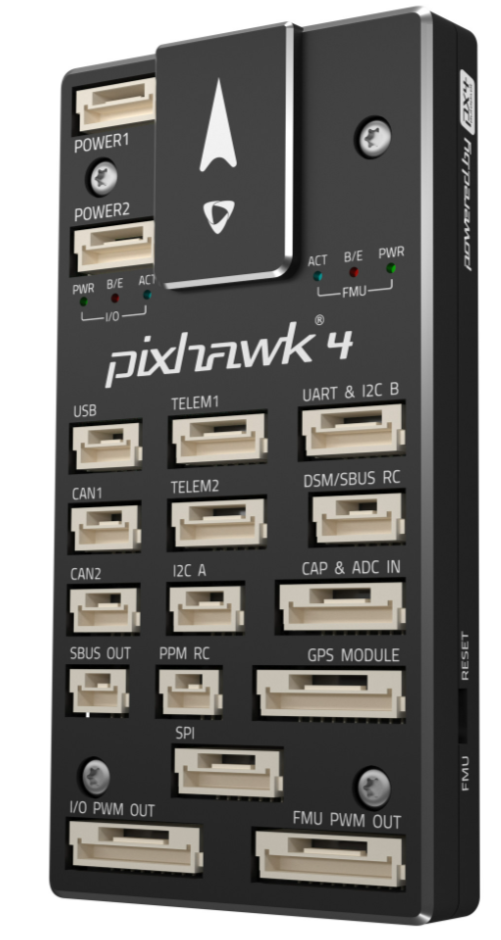
\includegraphics[scale=0.47]{obrazky/PIX}
    \end{center}
    \caption[Řídící jednotka Pixhawk 4]{Řídící jednotka Pixhawk 4 \cite{PIX2}.}
    \label{fig:PIX}
\end{figure}

\section{Palubní počítač}

Jako palubní počítač se pro experimentální letecké mise využívá jednodeskový počítač Raspberry PI. Na trhu existuje množství různých variant tohoto široce rozšířeného počítače v rozmezí od levného, malého a úsporného  \textit{Raspberry PI Pico} až po vysoce výkonný počítač \textit{Raspberry PI 4}.

Důležitými výhodami pro aplikace v robotických misích jsou integrace na jeden plošní spoj, nízká proudová spotřeba a možnost spuštění linuxových distribucí. Nejběžnější podporované distribuce jsou Raspberry PI OS, Raspbian, Ubuntu desktop a server.

Hlavní důvod pro použití Raspberry PI jako palubního počítače je možnost spolehlivé komunikace s PX4 firmware přes ROS 2 \textit{topic}. Komunikací mezi uvedenými platformami se budeme zabývat v následujících kapitolách.
\chapter{Firmware pro řízení bezpilotních letadel}

\section{BetaFlight}

BetaFlight je \textit{open-source} firmware pro řízení letu používaný k létání s multikoptérami a s letadly s pevnými křídly. Firmware se zaměřuje na letový výkon, špičkové funkce a širokou podporu platforem.

BetaFlight podporuje velkou škálu řídících jednotek, které mají alespoň \textit{STM32F4} procesor. Software pro nastavování parametrů (\textit{BetaFlight Configurator}) běží na Windows, Mac OS, Linux a Android.

Firmware Betaflight podporuje komunikaci s dálkovými ovládači od většiny výrobců, jako jsou FrSky, Graupner, Spektrum, DJI a FlySky. Řídící jednotku s BetaFlight firmware je možné povelovat i z nadřazeného systému pomocí \textit{\acs{MSP}} \footnote{\acs{MSP} (\acl{MSP}) je komunikační protokol pro posílání informací o telemetrii, dat ze snímačů a ovládání \cite{ARDU}}. \cite{BetaF}

\section{INAV}

INAV autopilot je odvozený od BetaFlight a zaměřuje se hlavně na autonomní lítání. Podporuje velké množstvi modelů od závodních a freestyle dronů, přez letadla až pod rovery a jiné kolové vozidla.

Firmware podporuje širokou škálu řídících jednotek od různých výrobců, podporuje zpracování dat ze senzorů a umožňuje ukládání dat o letu a vnitřním stavu dronu v reálném čase (\textit{blackbox}). \cite{INAV}

Software\textbf{} \textit{INAV Configurator} nabízí plánování \textit{waypoint} mise pro jakýkoliv autonomní model s řídící jednotkou, v které běží INAV firmware.

\section{Firmware pro řídící jednotku Pixhawk}

Existují dvě hlavní větve vývoje firmware pro řídící jednotku Pixhawk. Jednou platformou je open source projekt ArduPilot \cite{ARDU}, který podporuje velké množství bezpilotních prostředků a umožňuje vytváření autonomních misí. Druhým projektem je profesionální autopilot PX4 \cite{PX4ORG}. Velkou výhodou obou projektů je, že jsou do velké části kompatibilní, například software pro pozemní stanice QGroundControl z platformy PX4 může komunikovat s řídící jednotkou s firmware od ArduPilot a naopak. Vzájemná kompatibilita je zajištěna využitím stejného komunikačního protokolu MAVLink. Výhoda protokolu MAVLink spočívá aj v tom, že oba firmware můžou komunikovat s ROS (Robot Operating System) přes MAVROS\footnote{MAVROS je komunikační ovládač (\textit{driver}) pro komunikaci mezi ROS a autopiloty s MAVLink protokolem}

\subsection{ArduPilot}

ArduPilot je open source autopilot podporující mnoho typů vozidel, například multikoptéry, tradiční vrtulníky, letadla s pevnými křídly, čluny, ponorky, rovery a další. Projekt ArduPilot má společnou historii s PX4, ale v minulosti se tyto dva projekty oddělili. Proto mají oba projekty do velké míry podobné využití a míří na stejnou platformu.

Zdrojový kód projektu ArduPilot je vyvíjen širokým spektrem profesionálů a nadšenců, takže výhodou je velká komunita poskytující řešení na řadu problémů.

Frimware ArduPilot je založený na ChibiOS \acs{RTOS} (\acl{RTOS}). ArduPilot taky poskytuje možnost simulace letového kódu jak simulací \acs{SITL} (\acl{SITL}), tak simulací \acs{HITL} (\acl{HITL}). \cite{ARDU}

Pro další pokračování v práci jsme zvolili projekt PX4, takže další části budou pojednávat o firmware PX4.


\chapter{PX4 autopilot}

PX4 je profesionální autopilot, vyvinutý světovými vývojáři z průmyslu a akademické obce a podporovaný aktivní celosvětovou komunitou. Pohání všechny druhy vozidel od závodních a nákladních dronů až po pozemní vozidla a ponorky. 

\section{Architektura PX4}

PX4 firmware se skládá ze dvou hlavních vrstev:
\begin{itemize}
    \item Flight stack (letový zásobník)
    \begin{itemize}
        \item Letový zásobník je systém pro odhad a řízení letu.
    \end{itemize}
    \item PX4 middleware
    \begin{itemize}
        \item PX4 middleware je obecná robotická vrstva, která podporuje jakýkoli typ autonomního robota a poskytuje interní/externí komunikaci a integraci s hardware.
        \item Middleware navíc obsahuje simulační vrstvu, která umožňuje spuštění letového kódu PX4 na desktopovém operačním systému a ovládání počítačem modelovaného vozidla v simulovaném prostoru.\\
    \end{itemize}
\end{itemize}

Všechny podporované typy vozidel (drony, letadla, čluny, rovery, ponorky atd.) sdílejí jedinou kódovou základnu, která má následující vlastnosti: \cite{PX4main}

\begin{itemize}
    \item Veškerá funkčnost je rozdělena na vyměnitelné a opakovaně použitelné komponenty
    \item Komunikace probíhá pomocí asynchronního předávání zpráv
    \item Systém se dokáže vypořádat s různou pracovní zátěží\\
\end{itemize}

Na obrázku \ref{fig:PX4_Arch} je zobrazen diagram, který poskytuje podrobný přehled stavebních bloků PX4. Horní část diagramu obsahuje middlewarové bloky, zatímco spodní část zobrazuje komponenty letového zásobníku (\textit{flight stack}).

Moduly spolu komunikují prostřednictvím sběrnice \textit{publish-subscribe} s názvem \textit{uORB}. Hlavní výhody schématu \textit{publish-subscribe} v PX4 jsou následující:

\begin{itemize}
    \item Systém je asynchronní a aktualizuje se okamžitě, když jsou k dispozici nová data
    \item Všechny operace a komunikace jsou plně paralelní
    \item Systémová komponenta může zpracovávat data odkudkoli (globální datový prostor)
\end{itemize}

\begin{figure}[!ht]
    \begin{center}
        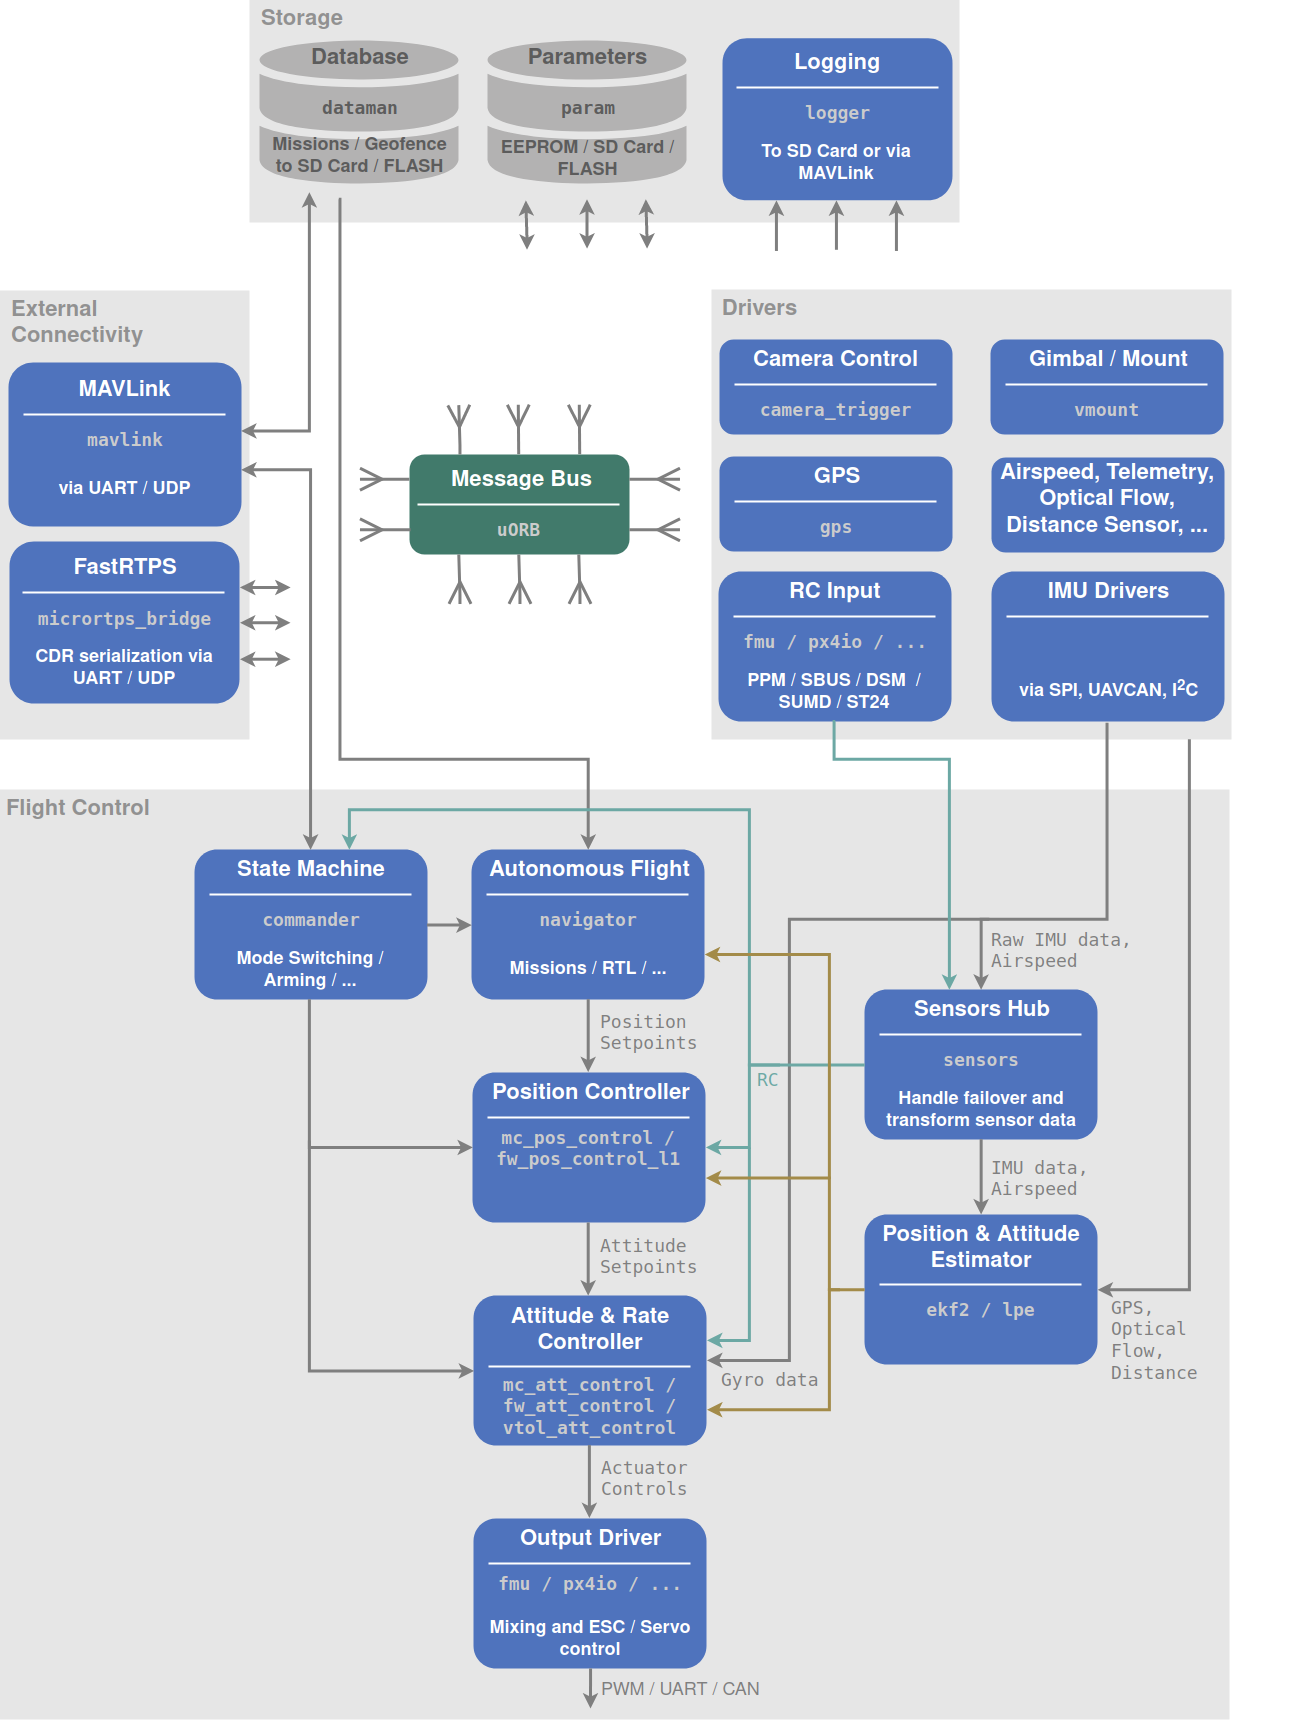
\includegraphics[scale=0.45]{obrazky/PX41}
    \end{center}
    \caption[Komplexní strukturální architektura PX4 software]{Komplexní strukturální architektura PX4 software \cite{PX4main}.}
    \label{fig:PX4_Arch}
\end{figure}

\subsection{PX4 jako samotný letový ovladač}

Na obrázku \ref{fig:PX4_FC} je naznačená architektura systému založeného na letovém ovladači (řídící jednotce) (\textit{flight controller}). Řídící jednotka zabezpečuje sběr dat ze senzorů, ovládání akčních členů dronu (pohony, serva, ...), řízení dronu na základě dat ze senzorů a povelů z RC rádia a v neposlední řadě stabilizaci dronu.

Do systému PX4 je možné zasílat povely z pozemní stanice (\textit{Ground Station}) přes protokol \textit{MAVlink} pomocí telemetrické rádiové soupravy.

\begin{figure}[!ht]
    \begin{center}
        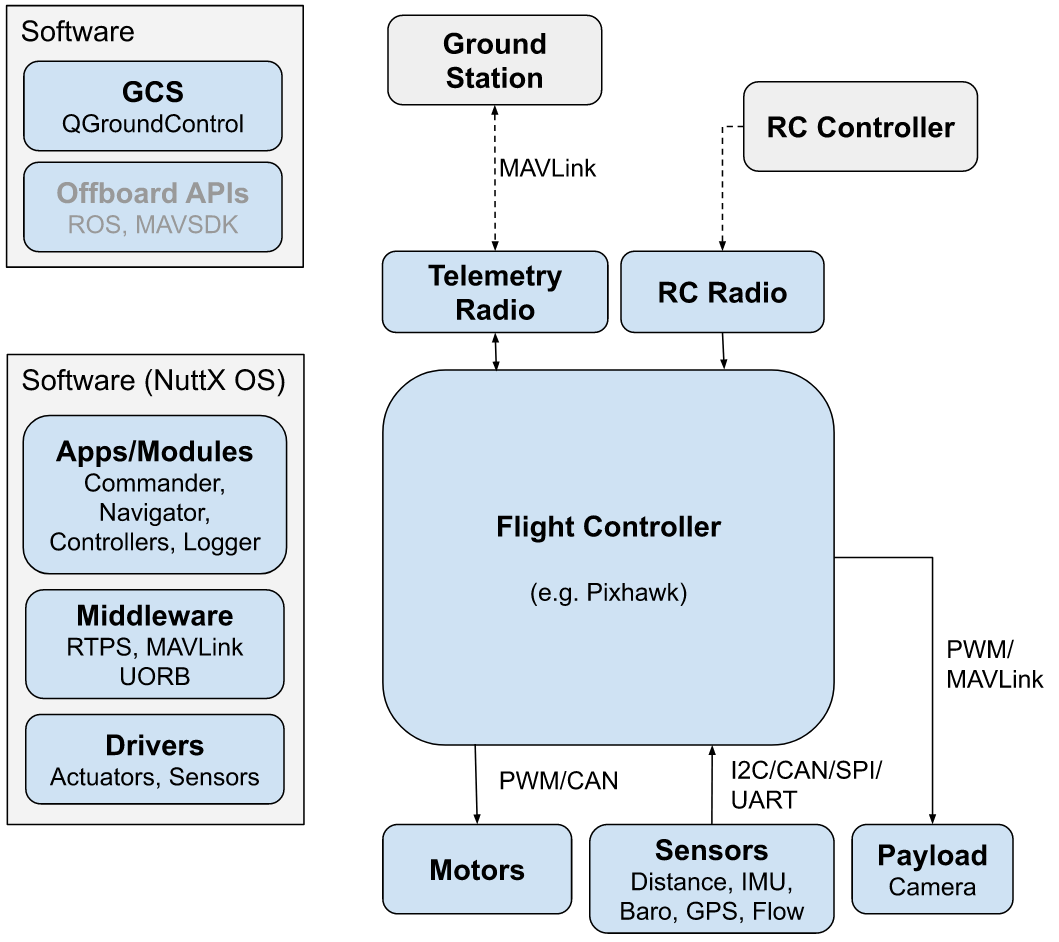
\includegraphics[scale=0.36]{obrazky/PX42}
    \end{center}
    \caption[Jednoduchý systém PX4 založený na letovém ovladači (flight controller)]{Jednoduchý systém PX4 založený na letovém ovladači (flight controller) \cite{PX4main2}.}
    \label{fig:PX4_FC}
\end{figure}

\subsection{Letový ovladač a počítač pro řízení mise}

Na obrázku \ref{fig:PX4_FC_PC} je zobrazená architektura systému PX4 založeného na letovém ovladači (řídící jednotce) a palubním počítači pro řízení mise. Řídící jednotka zabezpečuje sběr dat ze senzorů a ovládání akčních členů dronu (pohony, serva, ...). Komunikace mezi řídící jednotkou zabezpečuje protokol MAVlink, nebo \acs{RTPS} (\acl{RTPS}).

Palubní počítač pro řízení mise poskytuje pokročilé funkce, jako je vyhýbání se objektům a předcházení kolizím. Obvyklým operačním systémem je Linux s ROS (ROS 2) z důvodu, podpory knihoven na předcházení kolizím a z důvodu, že ROS 2 a PX4 využívají pro komunikaci s okolím \acs{DDS} (\acl{DDS}) middleware.

\begin{figure}[!ht]
    \begin{center}
        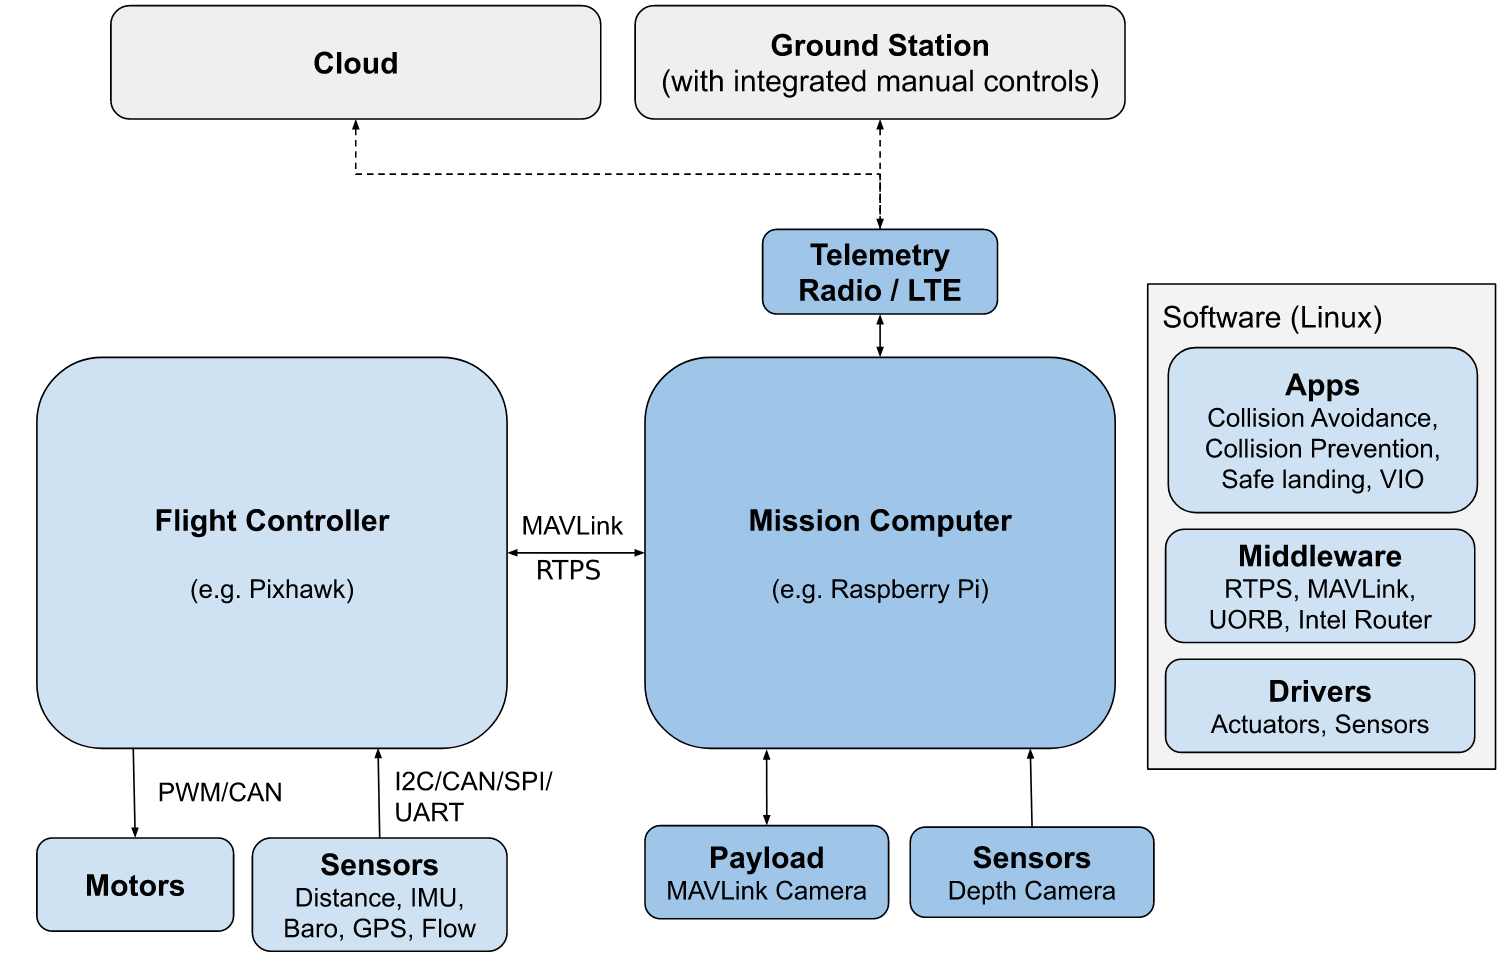
\includegraphics[scale=0.37]{obrazky/PX43}
    \end{center}
    \caption[Systém PX4 založený na letovém ovladači (flight controller) a palubním počítači pro řízení mise]{Systém PX4 založený na letovém ovladači (flight controller) a palubním počítači pro řízení mise \cite{PX4main2}.}
    \label{fig:PX4_FC_PC}
\end{figure}

\section{Licence}

Kód PX4 je zdarma k použití a úpravě za podmínek permisivní licence \textit{BSD 3-clause license} \cite{BSDlicense}.

Redistribuce a použití ve zdrojové a binární formě, s úpravami nebo bez nich, jsou povoleny za předpokladu, že jsou splněny následující podmínky:

1. Redistribuce zdrojového kódu musí obsahovat výše uvedenou poznámku o autorských právech, tento seznam podmínek a následující prohlášení o vyloučení odpovědnosti.

2. Redistribuce v binární formě musí reprodukovat výše uvedenou poznámku o autorských právech, tento seznam podmínek a následující prohlášení o vyloučení odpovědnosti v dokumentaci a/nebo jiných materiálech dodávaných s distribucí.

3. Jméno držitele autorských práv ani jména jeho přispěvatelů nesmí být použita k podpoře nebo propagaci produktů odvozených z tohoto software bez předchozího výslovného písemného povolení.

\section{QGround Control}

QGroundControl je software, který poskytuje plnou kontrolu letu a plánování mise pro jakýkoli dron s podporou MAVLink. Jeho primárním cílem je snadné použití pro profesionální uživatele a vývojáře. Veškerý kód je open source, takže je možné přispívat a dál ho vyvíjet \cite{QGround}.

Pomocí QGroundControl je možné nahrát nejnovější PX4, nebo Ardupilot firmware do letového ovladače (\textit{flight controller}), nastavit typ konstrukce dronu, ladit parametry regulace a vytvářet autonomní mise pomocí waypointů. Veškeré nastavení dronu a misí je jednoduché a velmi intuitivní.

Obrázek \ref{fig:QGC} zobrazuje základní obrazovku software QGroundControl.

\begin{figure}[!ht]
    \begin{center}
        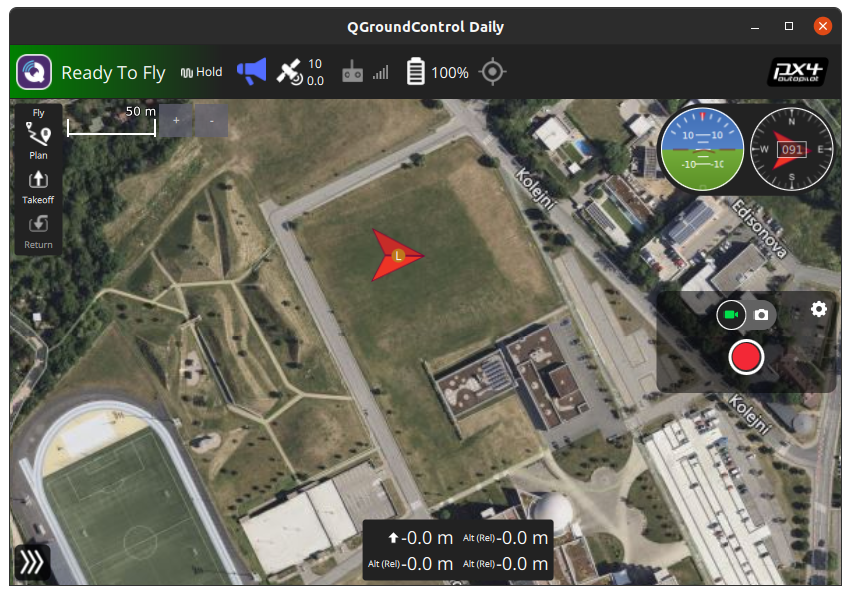
\includegraphics[scale=0.47]{obrazky/QG1}
    \end{center}
    \caption[Základní obrazovka QGroundControl]{Základní obrazovka QGroundControl.}
    \label{fig:QGC}
\end{figure}

Na základní obrazovce jsou zobrazeny stavové informace o dronu:

\begin{itemize}
    \item Relativní výška
    \item Azimut
    \item Orientace dronu (pitch, roll)
    \item RSSI (\textit{Received Signal Strength Indication})
    \item Počet připojených GPS satelitů
    \item Procento nabití akumulátoru
    \item Letový mód
\end{itemize}

\subsection{Nastavení konstrukce dronu}

Systém QGroundControl podporuje velké množství typů konstrukcí dronů, letadel, roverů a ponorek. Obrázek \ref{fig:QGC1} zobrazuje všechny podporované typy zařízení, které dokáže systém PX4 ovládat.

\begin{figure}[!ht]
    \begin{center}
        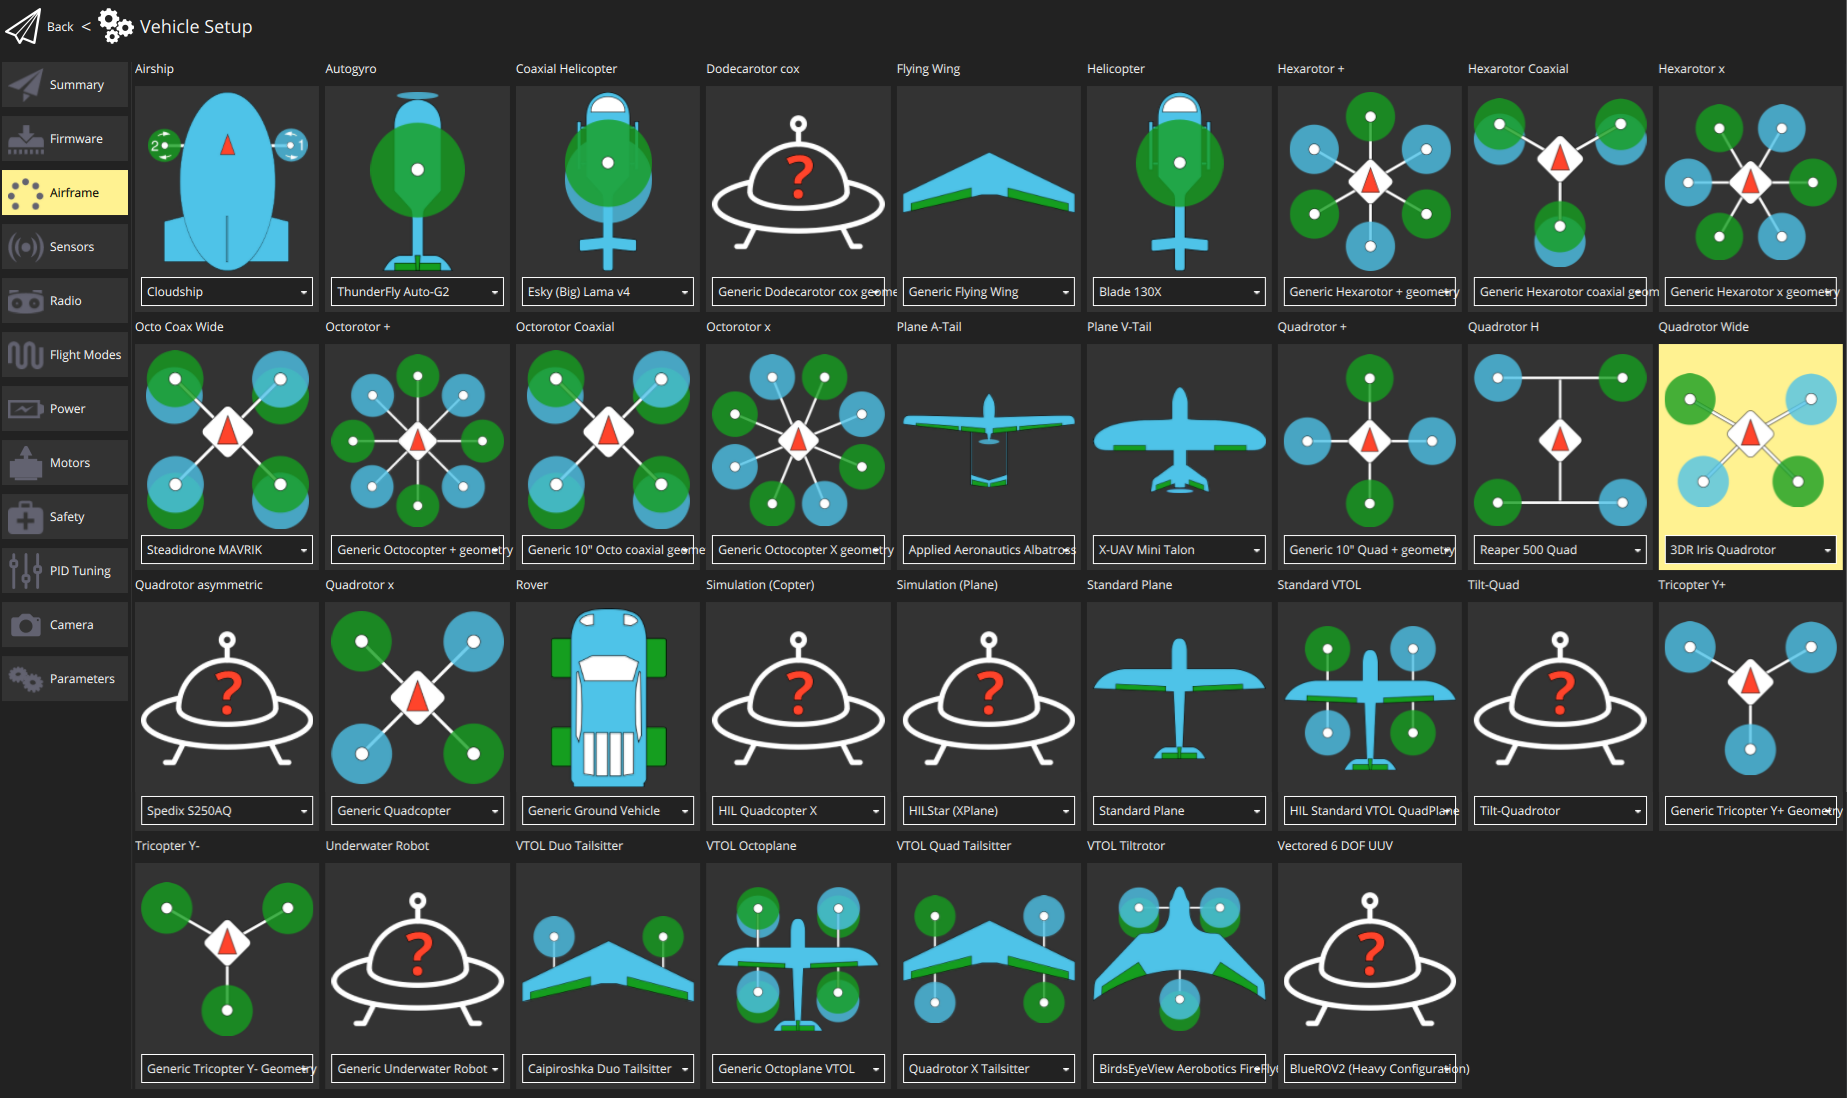
\includegraphics[scale=0.31]{obrazky/QG2}
    \end{center}
    \caption[Základní obrazovka QGroundControl]{Základní obrazovka QGroundControl.}
    \label{fig:QGC1}
\end{figure}

\subsection{Plánování bezpilotní mise}
\label{subs:planovani}

Software QGroundControl nabízí intuitivní plánování bezpilotních misí. Vlastní misi je možné naplánovat pomocí waypointů, nebo pomocí 3 přednastavených plánů pro bezpilotní mise: \cite{QGround2}

\begin{itemize}
    \item Průzkum prostředí
    \item Skenování koridoru
    \item Skenování konstrukcí
\end{itemize}

\subsubsection{Průzkum prostředí}

Pomocí tohoto plánu se vytvoří mřížkový letový vzor nad polygonální oblastí definovanou uživatelem. Oblast je možné definovat jako mnohoúhelník nebo kruh. Je zde taky možné nastavit mřížku přeletů, výšku nad povrchem jako absolutní, nebo relativní vůči terénu. Program umožňuje nastavení snímkování prostředí s podporou geotagging\footnote{Geotagging představuje přidávání geografických metadat k různým médiím jako jsou např.: obrázky.}. Obrázek \ref{fig:QGC2} zobrazuje nastavení autonomní mise s průzkumem prostředí.

\begin{figure}[!ht]
    \begin{center}
        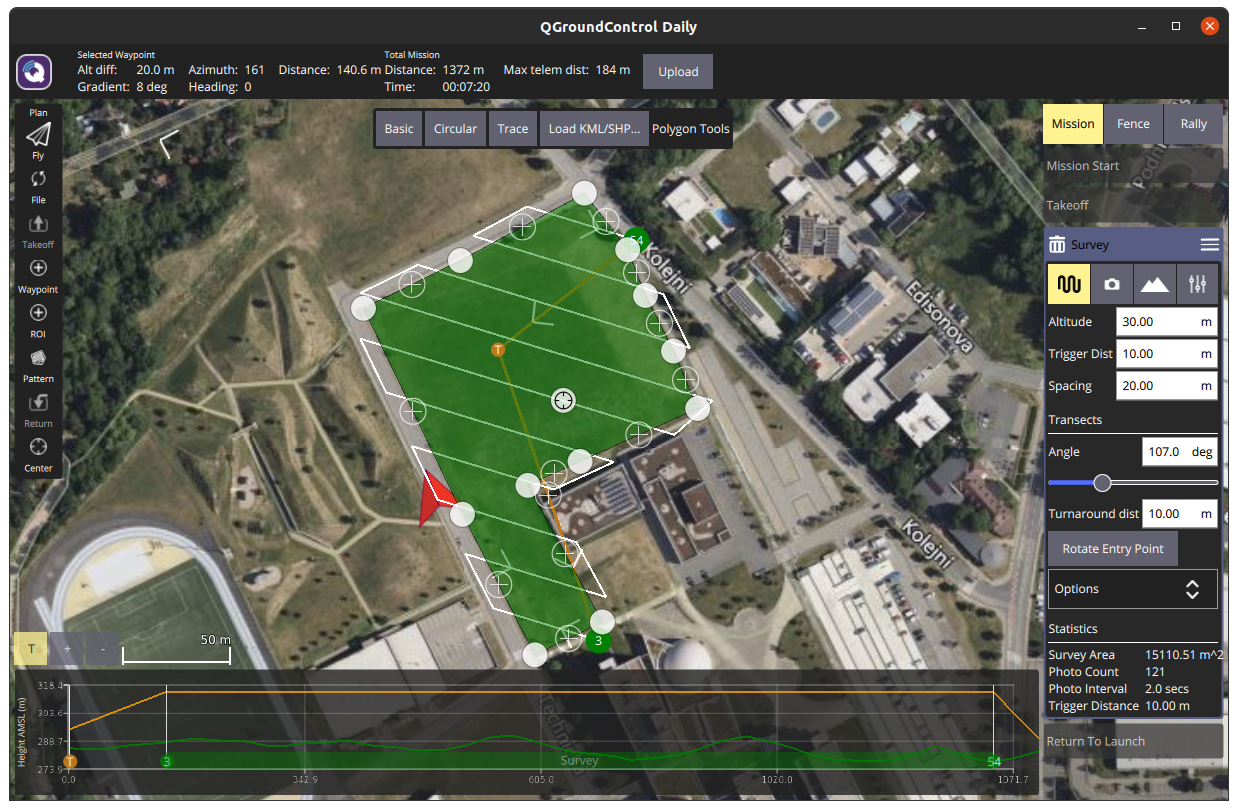
\includegraphics[scale=0.34]{obrazky/QGC3}
    \end{center}
    \caption[Nastavení bezpilotní mise pro průzkum prostředí]{Nastavení bezpilotní mise pro průzkum prostředí.}
    \label{fig:QGC2}
\end{figure}

\subsubsection{Skenování konstrukcí}

Pomocí plánu na skenování konstrukcí je možné naplánovat bezpilotní misi zaměřenou na snímkování svislých povrchů. Snímky se používají na vizuální kontrolu budov, nebo tvorbu 3D modelů konstrukcí. Obrys konstrukce je možné zadat jako mnohoúhelník nebo kruh. Dron bude oblétat celou budovu předem v nastavených výškách tak, aby kamera směřovala vždy na budovu. Po zadání konkrétní kamery, objektivu a rozlišení snímkování [cm/px] si program sám dopočítá vhodnou letovou vzdálenost od budovy a výšku jednotlivých letových vrstev. Na obrázku \ref{fig:QGC3} je zobrazeno nastavení autonomní mise pro skenování konstrukcí.

\begin{figure}[!ht]
    \begin{center}
        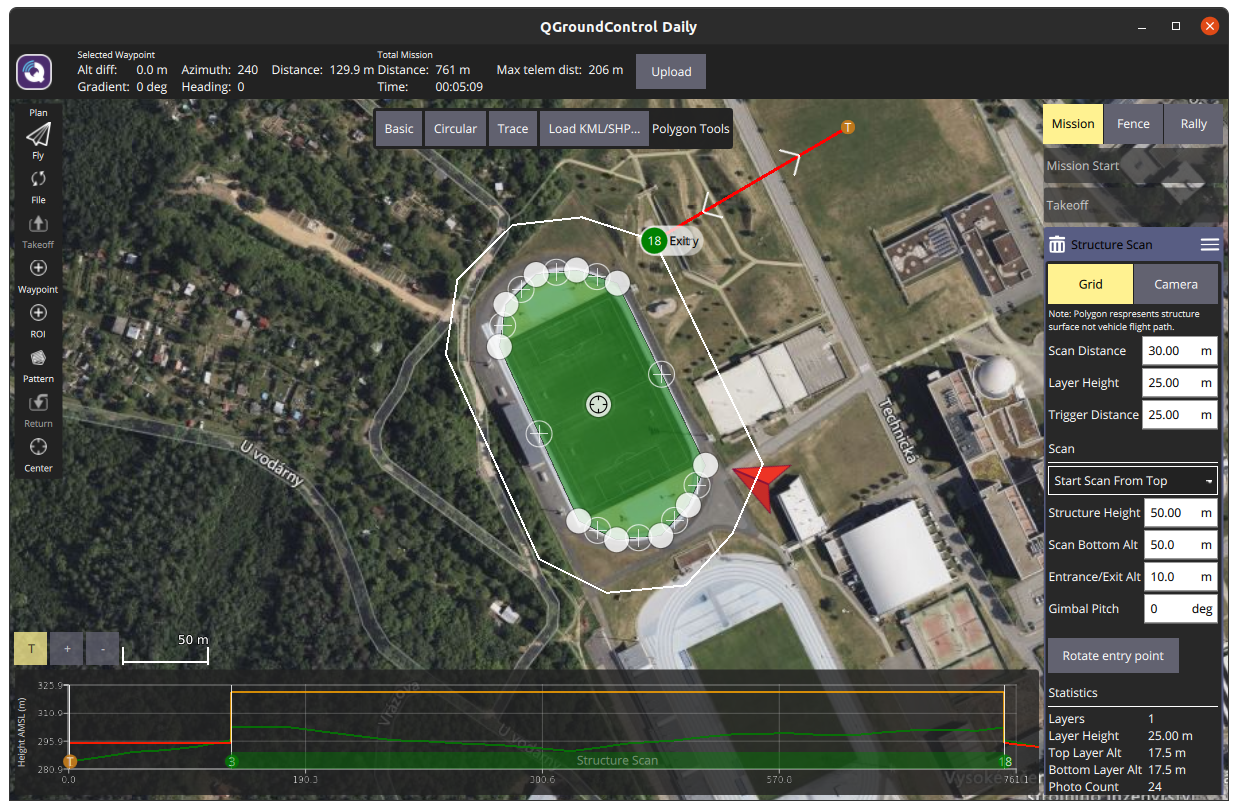
\includegraphics[scale=0.34]{obrazky/QGC5}
    \end{center}
    \caption[Nastavení bezpilotní mise pro skenování konstrukcí]{Nastavení bezpilotní mise pro skenování konstrukcí.}
    \label{fig:QGC3}
\end{figure}

\subsubsection{Skenování koridoru}

Letový plán pro skenování koridoru je vhodný pro sledování křivky (například pro průzkum silnice). Je možné si zde nastavit parametry letového vzoru jako jsou výška přeletu a hustota přeletů nad oblastí. Po zadání parametrů kamery a rozlišení snímkování [cm/px] si program sám dopočítá optimální letový vzor. Obrázek \ref{fig:QGC4} zobrazuje nastavení letového plánu pro skenování koridoru.

\begin{figure}[!ht]
    \begin{center}
        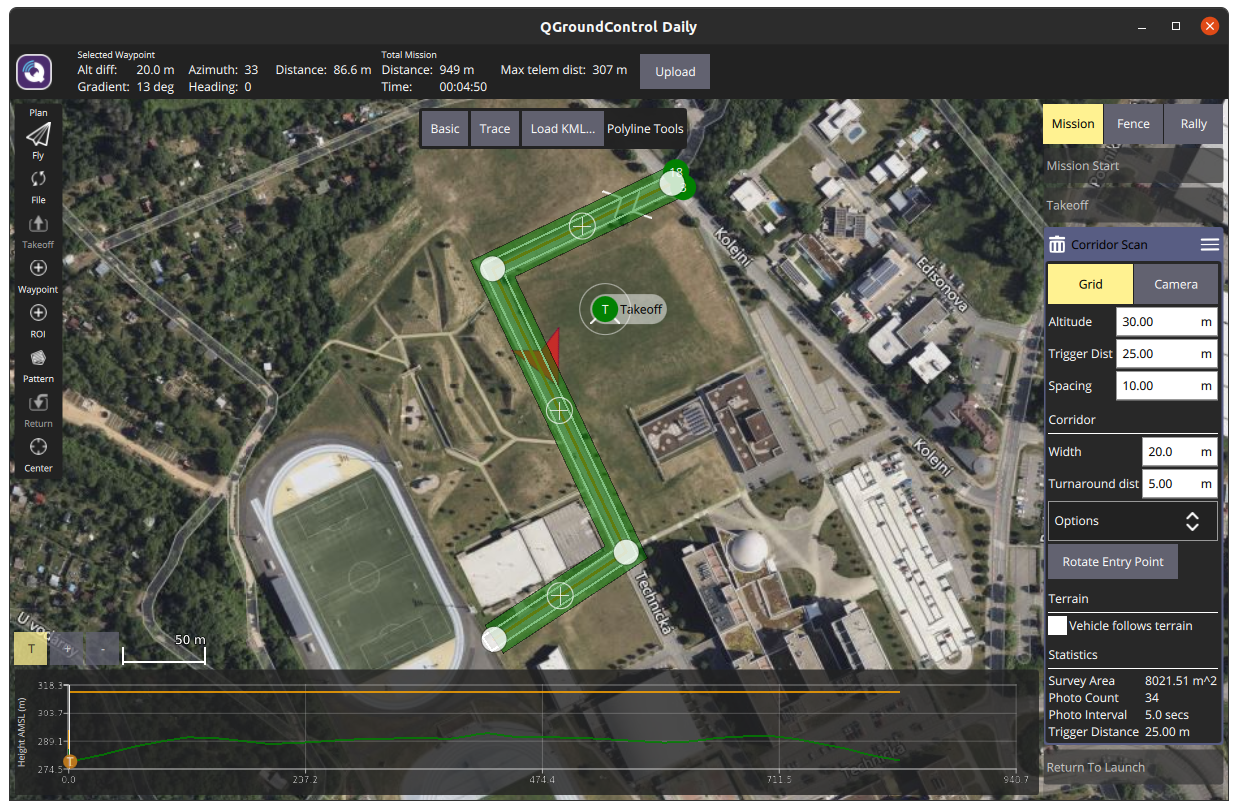
\includegraphics[scale=0.34]{obrazky/QGC4}
    \end{center}
    \caption[Nastavení bezpilotní mise pro skenování koridoru]{Nastavení bezpilotní mise pro skenování koridoru.}
    \label{fig:QGC4}
\end{figure}


\chapter{Propojení PX4 a ROS 2}

Existuji dva hlavní přístupy pro výměnu dat mezi ROS 2 middleware a PX4 firmware:

\begin{itemize}
    \item Přímá komunikace s využitím \acs{DDS} middleware
    \item Komunikace pomocí MAVLink protokolu\\
\end{itemize}

V následující kapitole jsou detailně popsány obě možnosti komunikace.

\section{Komunikace pomocí pomocí DDS\texorpdfstring{\textsuperscript{\textregistered}}{ (R)}}

\subsection{Struktura komunikace v ROS 2}

Velká změna, která se udála v ROS ekosystému při přechodu z ROS na ROS 2 bylo zvolení \acs{DDS} (\acl{DDS}) middleware jako hlavního komunikačního prostředku.

Každý ROS 2 uzel (\textit{node}) je namapovaný do vlastního \acs{DDS} procesu. Pokud je spuštěno více ROS 2 uzlů, tak každý uzel je namapovaný do samostatného \acs{DDS} procesu. \cite{ROS2DDS3}

\subsection{Vnitřní komunikace v PX4}

\textit{uORB} je asynchronní \acs{API} pro zasílání zpráv \textit{publish} a \textit{subscribe} používané pro komunikaci mezi vlákny a procesy PX4. \textit{uORB} \acs{API} je automaticky spuštěno při startu PX4 systému, protože na něm závisí množství vnitřních procesů PX4.

V systému PX4 je definovaných 167 \textit{uORB} zpráv. Úplný seznam je zveřejněný v uživatelském manuálu PX4: \url{https://docs.px4.io/master/en/msg_docs/} \cite{PX4docs}

\subsection{MicroRTPS agent a klient}
\label{sec:komunikace}

PX4-Fast RTPS(\acs{DDS} ) Bridge, který je také označován jako microRTPS Bridge, přidává k PX4 Autopilot rozhraní \acs{RTPS} (\acl{RTPS}), které umožňuje výměnu zpráv \textit{uORB} mezi různými interními komponenty PX4 a \uv{mimo-palubní} komunikaci s \acs{DDS} aplikacemi v reálném čase.

\acs{RTPS} umožňuje lepší integraci s aplikacemi spuštěnými a propojenými v doménách \acs{DDS} (včetně uzlů ROS 2), což usnadňuje sdílení dat ze senzorů, příkazů a dalších informací o dronu.

Vhodným případem použití \acs{RTPS} jsou aplikace, kde je nutné komunikovat časově kritické informace (informace v reálném čase) mezi letovým ovladačem a \uv{mimo-palubními} (\textit{offboard}) komponenty. \acs{RTPS} je užitečný, kdy je mimo-palubní software kritický pro bezpilotní misi a rovnocenný s procesy běžící v PX4. Mezi možné příklady použití patří komunikace s uzly v ROS 2, které pracují s daty v reálném čase a jsou nezbytné pro ovládání dronu.

Výhoda \acs{RTPS} oproti protokolu MAVlink je v tom, že dokáže komunikovat na vyšších frekvencích. \cite{PX4docs}

\subsubsection{MicroRTPS klient}

MicroRTPS klient je \textit{deamon}, který běží na řídící jednotce (\textit{flight controller}) PX4. Klient se přihlásí k odběru (\textit{subscribe}) zpráv \textit{uORB} publikovanými interními komponenty autopilota PX4 a odesílá zprávy agentovi (přes UART nebo UDP). Klient taky přijímá zprávy od agenta a publikuje je jako \textit{uORB} zprávy do systémy PX4. \cite{PX4docs}

\subsubsection{MicroRTPS agent}

MicroRTPS agent běží jako \textit{deamon} na palubním počítači. Agent sleduje aktualizační \textit{uORB} zprávy od klienta a publikuje je přes \acs{RTPS} do \acs{DDS} domény. Agent taky přijímá zprávy strukturované jako \textit{uORB} z jiných aplikací v \acs{DDS} doméně a přeposílá je klientovi.

\subsubsection{Komunikace mezi microRTPS agentem a klientem}

Jak je zobrazeno na obrázku \ref{fig:RTPS_a_c} agent a klient jsou propojeni přes sériovou linku (UART) nebo UDP síť a informace \textit{uORB} jsou serializovány pomocí \acs{CDR} (\acl{CDR})\footnote{\acl{CDR} je způsob nízkoúrovňové serializace dat mezi různými platformami \cite{CDR}} před odesláním. Micro RTPS agent a všechny \acs{DDS} aplikace jsou propojeny přes UDP a mohou být na stejném nebo jiném zařízení.

\begin{figure}[!ht]
    \begin{center}
        \hspace*{-1cm}
        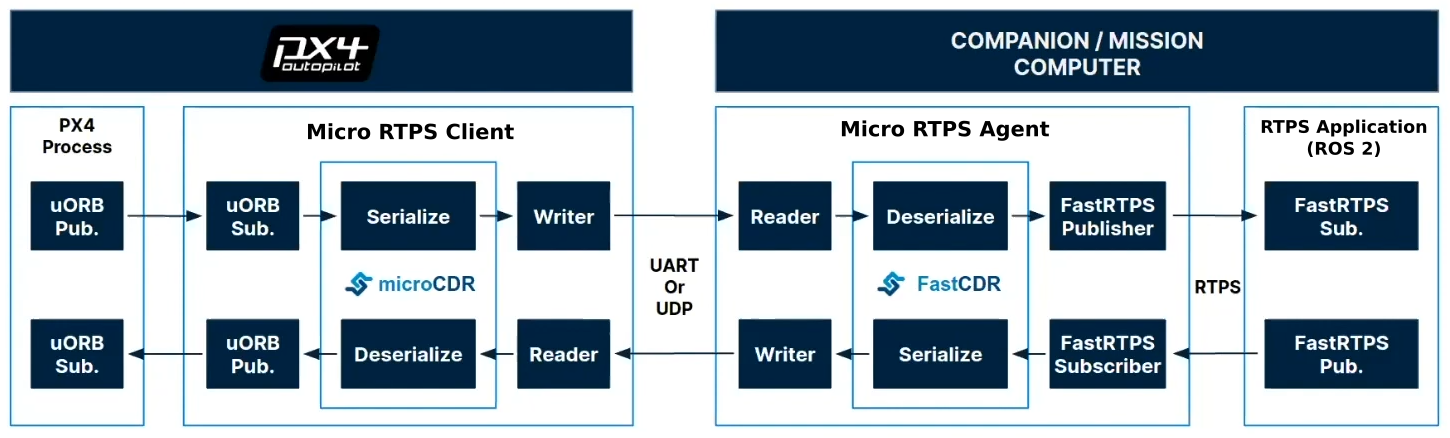
\includegraphics[scale=0.45]{obrazky/RTPS1}
    \end{center}
    \caption[Schéma komunikace mezi microRTPS agentem a klientem]{Schéma komunikace mezi microRTPS agentem a klientem. \cite{PX4docs}}
    \label{fig:RTPS_a_c}
\end{figure}

\subsection{DDS\texorpdfstring{\textsuperscript{\textregistered}}{ (R)} / RTPS middleware}

Služba OMG\footnote{Object Management Group\textsuperscript \textregistered (OMG\textsuperscript \textregistered) je mezinárodní neziskové konsorcium pro technologické standardy s otevřeným členstvím.} Data-Distribution Service for Real-Time Systems\textsuperscript \textregistered (\acs{DDS}) je prvním otevřeným mezinárodním middlewarovým standardem, který přímo řeší komunikaci pro \textit{publish and subscribe} systémy v reálném čase.

\acs{DDS} představuje virtuální globální datový prostor, kde mohou aplikace sdílet informace pouhým čtením a zápisem datových objektů. Datové objekty jsou adresované pomocí definovaného názvu (\textit{topic}) a klíče (\textit{key}). \acs{DDS} integruje součásti systému dohromady a poskytuje datovou konektivitu s nízkou latencí, extrémní spolehlivost a škálovatelnou architekturu. Nabízí rozsáhlé řízení parametrů \acs{QoS} (\acl{QoS}), včetně spolehlivosti, šířky pásma a limitů zdrojů \cite{DDS_Def}. 

\acs{DDS} middleware komunikuje \textit{peer-to-peer} a nevyžaduje, aby byla data zprostředkována serverem nebo cloudem. 

Jak je zobrazeno na obr \ref{fig:DDSmiddleware}, \acs{DDS} middleware je software vrstva, která odděluje aplikaci od detailů operačního systému, síťového přenosu a nízkoúrovňových datových formátů. Nízkoúrovňové detaily, jako je formát dat v paměti, spolehlivost, protokoly, výběr přenosového kanálu, \acs{QoS}, zabezpečení atd. jsou spravovány middlewarem. 

\begin{figure}[!ht]
    \begin{center}
        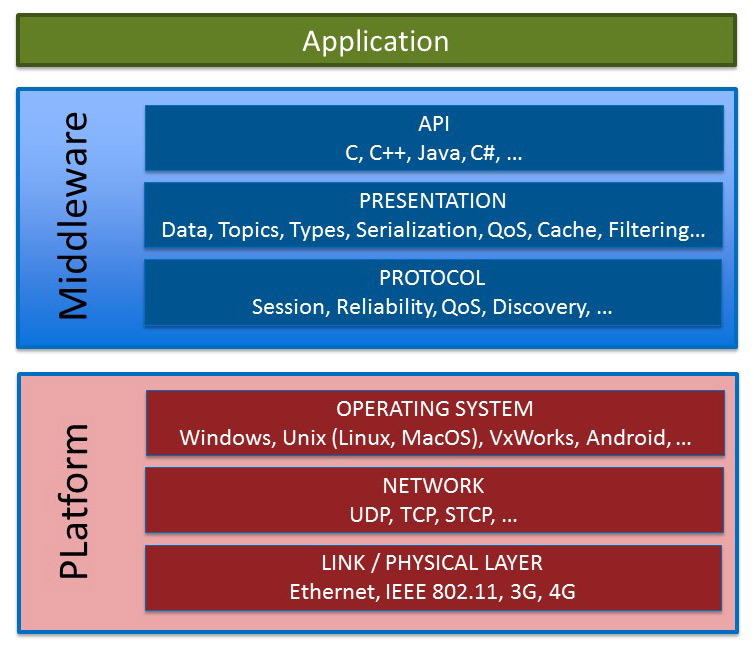
\includegraphics[scale=0.4]{obrazky/DDS1}
    \end{center}
    \caption[Propojení \acs{DDS} middlewaru s aplikací a operačním systémem]{Propojení \acs{DDS} middlewaru s aplikací a operačním systémem \cite{DDS_Main}.}
    \label{fig:DDSmiddleware}
\end{figure}

\subsubsection{DDS\texorpdfstring{\textsuperscript{\textregistered}}{ (R)} a ROS 2}

\acs{DDS} middleware je základní komunikační interface pro ROS 2. Middleware zajišťuje dynamické hledání bodů v síti, serializaci a \textit{publish/subscribe} přenos dat. ROS 2 skrývá velkou část složitosti \acs{DDS} pro většinu uživatelů, ale taky poskytuje přístup k základní implementaci \acs{DDS} pro uživatele, kteří potřebují vyřešit extrémní případy nebo potřebují integraci s jinými stávající \acs{DDS} systémy. \cite{ROS2DDS}

ROS 2 podporuje více implementací \acs{DDS}/RTPS. Při výběru implementace middlewaru můžete zvážit mnoho faktorů, jako je licence, dostupnost platformy nebo výpočetní náročnost. Existují varianty middleware, které jsou vytvořeny pro mikrokontroléry, nebo varianty, které se zaměřují na aplikace vyžadující speciální bezpečnostní certifikace.

Podpora několika implementací \acs{DDS} middleware je důležitá pro zajištění toho, aby kódová základna ROS 2 nebyla vázána na žádnou konkrétní implementaci, protože uživatelé mohou chtít implementace přepínat v závislosti na potřebě jejich projektu. \cite{ROS2DDS2}

ROS 2 podporuje tyto \acs{DDS} implementace:
\begin{itemize}
    \item RTI (Real-Time Innovations) Connext
    \item Eclipse Cyclone DDS
    \item eProsima Fast DDS
\end{itemize}

\subsection{Základní principy DDS\texorpdfstring{\textsuperscript{\textregistered}}{ (R)}}
\subsubsection{Orientace na data (data centricity)}

\acs{DDS} middleware je jeden z mála middleware, který je zaměřen na data. Orientace na data zajišťuje, že všechny zprávy obsahují správné kontextové informace, které aplikace potřebuje k pochopení dat, která přijímají.

Podstatou orientace na data je, že \acs{DDS} middleware má informaci o tom, jaká data ukládá, a řídí, jak tato data sdílet. Programátoři používající tradiční middleware zaměřený na zprávy musí napsat kód, který odesílá zprávy. Programátoři používající middleware orientovaný na data píší kód, který určuje, jak a kdy sdílet data a poté přímo sdílejí datové hodnoty. \acs{DDS} přímo implementuje řízené, spravované a bezpečné sdílení dat. \cite{DDS_Main}

\subsubsection{Globální datový prostor}

\acs{DDS} aplikace má přístup k lokálnímu úložišti dat nazývanému \textit{globální datový prostor}. \textit{Globální datový prostor} vypadá pro aplikaci jako lokální paměť přístupná přes \acs{API} (\acl{API}). \acs{DDS} middleware posílá zprávy k aktualizaci příslušných úložišť na vzdálených komunikačních uzlech (\textit{nodes}).

V \acs{DDS} aplikacích neexistuje žádné globální datové místo, kde by všechna data existovala. Každá aplikace si lokálně ukládá jen to, co potřebuje a jen tak dlouho, jak to potřebuje. \cite{DDS_Main}

\acs{DDS} se zabývá daty v pohybu - globální datový prostor je virtuální koncept, který je ve skutečnosti pouze souborem lokálních úložišť. Každá aplikace, téměř v jakémkoli jazyce, běžící na jakémkoli systému, vidí lokální paměť ve svém optimálním nativním formátu. Globální datový prostor sdílí data mezi vestavěnými, mobilními a cloudovými aplikacemi v rámci jakéhokoli přenosu, bez ohledu na jazyk nebo systém, a s extrémně nízkou latencí.

\subsubsection{Základní architektura DDS\texorpdfstring{\textsuperscript{\textregistered}}{ (R)}}

Nejzákladnějším komunikačním vzorem podporovaným \acs{DDS} je model publikování/přihlášení (\textit{Publish/Subscribe}). \textit{Publish/Subscribe} je komunikační model, kde producenti dat publikují data a spotřebitelé dat se přihlašují k odběru dat. Tito producenti a spotřebitelé o sobě nemusí vědět předem, protože se navzájem dynamicky objevují za běhu. Data, která sdílejí, jsou popsána tématem (\textit{topic}) a producenti a spotřebitelé odesílají a přijímají data pouze pro témata, která je zajímají. V tomto vzoru může mnoho producentů publikovat stejné téma a mnoho spotřebitelů se může přihlásit k odběru stejného tématu. Spotřebitelé dostávají data od všech producentů, se kterými sdílejí téma. Producenti odesílají data přímo Spotřebitelům, aniž by potřebovali brokera nebo centralizovanou aplikaci pro zprostředkování komunikace. \cite{DDS_PubSub}

Jak je zobrazeno na obrázku \ref{fig:DDSarch} v \acs{DDS} se objekty, které publikují data, nazývají \textit{DataWriters} a objekty, které odebírají data, jsou \textit{DataReaders}. \textit{DataWriters} a \textit{DataReaders} jsou spojeni s jedním objektem \textit{Topic}, který tato data popisuje.

\begin{figure}[!ht]
  \begin{center}
    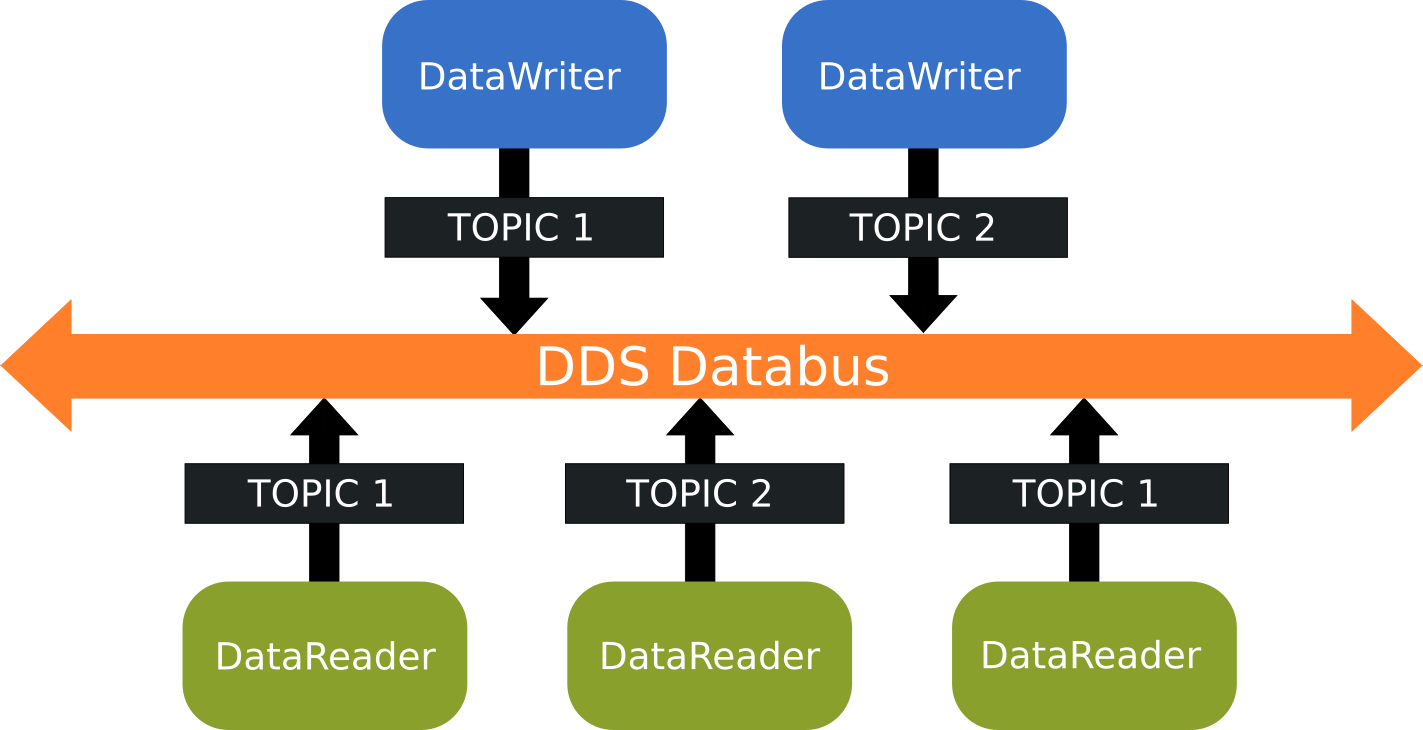
\includegraphics[scale=0.35]{obrazky/DDS2}
  \end{center}
  \caption[Základní \textit{publish/subscribe} struktura \acs{DDS} komunikace]{Základní \textit{publish/subscribe} struktura \acs{DDS} komunikace \cite{DDS_PubSub}.}
  \label{fig:DDSarch}
\end{figure}

\subsubsection{Quality of Service}

V \acs{DDS} aplikacích je možné sdílet data s flexibilními specifikacemi kvality služeb (\acs{QoS}), jako jsou spolehlivost, stav systému, živost, zabezpečení a mnohé další. 

\acs{DDS} middleware posílá jen data, které jsou nutné pro správnou funkci systému. Pokud se zprávy nedostanou do zamýšlených cílů, middleware automaticky zvýší spolehlivost na daných datových cestách. Když se komunikační systémy změní, middleware dynamicky zjistí, kam poslat data, a informuje účastníky o změnách. Pokud je celková velikost dat obrovská, \acs{DDS} inteligentně filtruje a odesílá pouze data, která každý koncový bod skutečně potřebuje a tím snižuje nároky na komunikační kanál. Když je potřeba, aby byly aktualizace rychlé, \acs{DDS} odesílá multicastové zprávy pro aktualizaci mnoha vzdálených aplikací najednou. U aplikací kritických z hlediska zabezpečení \acs{DDS} řídí přístup, vyhodnocuje cesty toku dat a šifruje data za běhu. \cite{DDS_Main}

\subsubsection{\acs{RTPS} protokol}

\acs{DDSI} (\acl{DDSI}), jinak \acs{RTPS} (\acl{RTPS}) je protokol pro spolehlivou komunikaci \textit{publish/subscribe} přes nespolehlivé přenosy, jako je UDP pro unicast i multicast. \cite{DDS_Standard}

\acs{RTPS} byl standardizován OMG (Object Management Group) jako protokol pro implementaci \acl{DDS} (\acs{DDS}), standard široce používaný v leteckém a obranném sektoru pro aplikace v reálném čase.

Kromě implementací \acs{RTPS} zabudovaných do různých implementací \acs{DDS} existují samostatné lehké implementace \acs{RTPS} (eProsima Fast \acs{RTPS}).

Protokol RTPS je založen na různých modulech, které řídí výměnu informací mezi různými \acs{DDS} aplikacemi: \cite{Eprosima}

\begin{itemize}
    \item \textit{Structure module} - definuje komunikační koncové body (\textit{endpoints}) a mapuje je na jejich protějšky \acs{DDS}.
    \item \textit{Message module} - definuje, které zprávy si mohou tyto koncové body vyměňovat a jak jsou sestaveny.
    \item \textit{Behavior module} - definuje sadu povolených interakcí a jejich vliv na každý z koncových bodů.
    \item \textit{Discovery module} - definuje sadu vestavěných koncových bodů, které umožňují automatické zjišťování.
\end{itemize}

\subsubsection{Dynamické hledání bodů v síti}

\acs{DDS} poskytuje dynamické zjišťování producentů a spotřebitelů dat. Dynamické hledání umožňuje rozšiřitelnost všech \acs{DDS} aplikací. To znamená, že aplikace nemusí znát nebo konfigurovat koncové body pro komunikaci, protože je automaticky za běhu zjistí \acs{DDS}.

Při dynamickém hledání bodů v síti \acs{DDS} zjistí, zda koncový bod publikuje data, odebírá data nebo obojí. Zjistí typ dat, která jsou publikována nebo odebírána. Zjistí také komunikační charakteristiky nabízené producentem a komunikační charakteristiky požadované spotřebitelem dat. Všechny tyto atributy jsou brány v úvahu při dynamickém zjišťování a párování účastníků \acs{DDS}. \cite{DDS_Main}

Účastníci \acs{DDS} komunikace mohou být na stejném počítači nebo v síti. Není potřeba znát nebo konfigurovat IP adresy nebo brát v úvahu rozdíly v architektuře strojů, takže přidání dalšího účastníka komunikace je snadné.

\subsection{Využití DDS\texorpdfstring{\textsuperscript{\textregistered}}{ (R)} v praxi}

\acl{DDS} je základem některých průmyslových standardů: \cite{DDS_usage}

\begin{itemize}
    \item OpenFMB (Open Field Message Bus)
    \item Adaptive AUTOSAR (AUTomotive Open System ARchitecture)
    \item MD PnP (Medical Device \uv{Plug-and-Play})
    \item GVA (Generic Vehicle Architecture)
    \item NGVA (NATO Generic Vehicle Architecture)
    \item ROS2 (Robot Operating System 2) \\[0.2cm]
\end{itemize}

\acs{DDS} má rozsáhlý seznam různých instalací, které jsou často kritické. \cite{ROS2DDS}

\begin{itemize}
    \item Bitevní lodě
    \item Velké inženýrské instalace, jako jsou přehrady
    \item Finanční systémy
    \item Vesmírné systémy
    \item Letové systémy
    \item Systémy vlakových rozvaděčů
\end{itemize}

\section{Komunikace pomocí MAVLink}

MAVLink (\textit{Micro Air Vehicle communication protocol}) je \uv{lehký} protokol využívaný už od roku 2009 pro komunikaci mezi vnitřními procesy na palubě dronu, nebo mezi pozemní stanicí a dronem v náročných komunikačních podmínkách jako je vysoká latence, nebo šum prostředí.

Základní komunikační schémata využívána protokolem MAVLink jsou \textit{publish-subscribe} a \textit{point-to-point}.

Knihovny, které implementují funkce a definují zprávy MAVLink protokolu, jsou pro většinu programovacích jazyků vydány s MIT licencí, takže je lze bez omezení využívat v libovolné aplikaci s uzavřeným zdrojovým kódem. Proto je možné MAVLink protokol využívat na různých platformách, jako jsou Windows, Linux, iOS a Android, ale i na mikrokontrolérech včetně ARM7, ATMega, dsPic, STM32. \cite{MAVLINK}

\subsection{MAVLink zprávy}

Společná sada zpráv MAVLink obsahuje standardní definice, které jsou spravovány protokolem MAVLink. Tyto definice zahrnují hlavně funkce, které jsou považovány za užitečné pro většinu pozemních řídicích stanic a autopilotů. Od všech systémů kompatibilních s protokolem MAVLink se očekává, že budou tyto definice používat tam, kde je to možné.

Seznam standardních definic zpráv protokolu MAVLink je zveřejněn zde: \url{https://mavlink.io/en/messages/common.html}

Na obrázku \ref{fig:MAV1} je zobrazena struktura MAVLink zprávy.

\begin{figure}[!ht]
  \begin{center}
    \hspace*{-1cm}
    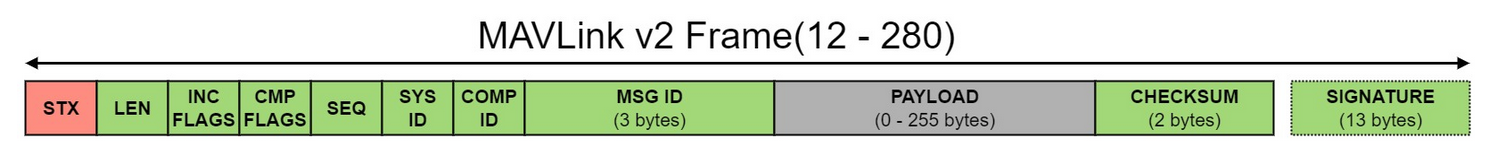
\includegraphics[scale=0.31]{obrazky/MAV1}
  \end{center}
  \caption[Strura MAVLink zprávy]{Strura MAVLink zprávy \cite{MAVLINK}.}
  \label{fig:MAV1}
\end{figure}

\begin{itemize}
    \item \texttt{STX}: Indikace začátku paketu (hodnota \texttt{0xFD})
    \item \texttt{LEN}: Délka sekce s datama - \texttt{PAYLOAD}
    \item \texttt{INC FLAGS}: Příznak nekompatibility
    \begin{itemize}
        \item Definuje kritické funkce, které musí daná implementace MAVLinku podporovat, aby bylo možné zpracovat paket.
    \end{itemize}
    \item \texttt{CMP FLAGS}:Příznak kompatibility
    \begin{itemize}
        \item Obsahuje doplňující informace, které nejsou nutné k správnému zpracování paketu.
    \end{itemize}
    \item \texttt{SEQ}: Pořadové číslo paketu pro zprávy skládající se z víc paketů
    \item \texttt{SYS ID}: Číslo systému v síti (vozidlo)
    \item \texttt{COMP ID}: Číslo komponenty na definovaném systému (kamera, autopilot, ...)
    \item \texttt{MSG ID}: Číslo zprávy
    \item \texttt{PAYLOAD}: Data
    \begin{itemize}
        \item Struktura dat je definována číslem zprávy (\texttt{MSG ID})
    \end{itemize}
    \item \texttt{CHECKSUM}: Informace pro detekci, jestli zpráva dorazila v pořádku
    \item \texttt{SIGNATURE}: Podpis, který zajisti zprávu proti neoprávněné manipulaci
\end{itemize}

\subsection{MAVLink mikroslužby}

MAVLink mikroslužby definují protokoly vyšší úrovně, pomocí kterých mohou systémy MAVLink komunikovat s vyšší efektivitou. Například pozemní stanice (QGroundControl, ArduPilot) a autopilot PX4 sdílejí společný příkazový protokol pro zasílání zpráv vyžadující potvrzení (\textit{acknowledge}).

Mikroslužby zajišťují, jak se rozdělí a znovu sestaví data, které mají většív velikost, než je velikost jedné zprávy. Jestliže jsou nějaká data ztracena v průběhu přenosu, mikroslužby iniciují opětovné odeslání dat.

Většina mikroslužeb využívá vzor \textit{client-server}, například pozemní stanice (klient) iniciuje požadavek a vozidlo (server) odpovídá daty.

\subsection{Využití protokolu MAVLink}

Velké množství autopilotů, pozemních stanic, \acs{API}, projektů a dalších softwarových balíčků používá protokol MAVLink.

\subsubsection{Autopilot}

Na trhu existuje velké množství hobby autopilotů, nebo profesionálních řešení pro modely letadel a dronů. Níže uvedený seznam zobrazuje aktivní vyvíjené autopiloty, které využívají komunikační MAVLink protokol.  \cite{MAVLINK}

\begin{itemize}
    \item PX4
    \item ArduPilot
    \item AutoQuad 6 AutoPilot
    \item iNAV
    \item SmartAP Autopilot\\
\end{itemize}


\begin{multicols}{2}
[
\subsubsection{Pozemní stanice}
]
    \begin{itemize}
        \item QGroundControl
        \item AutoQuad GCS
        \item SmartAP GCS
        \item Yuneec Datapilot
        \item Sentera Groundstation
        \item WingtraPilot
        \item APM Planner 2.
        \item Mission Planner
        \item MAVProxy
        \item UgCS (Universal Ground Control Station)
        \item Side Pilot
        \item JAGCS
        \item Flightzoomer
        \item Inexa Control
        \item Synturian Control
    \end{itemize}
\end{multicols}

\subsubsection{API}

Pro zjednodušení interakce s autopiloty, kamerami, pozemními stanicemi a mnoha dalšíma uzly s podporou MAVLink protokolu bylo vytvořeno několik vysokoúrovňových \acs{API}. Tyto \acs{API} poskytují implementace hlavních mikroslužeb a jednoduché komunikační rozhraní pro odesílání příkazů a k příjmu informací o vozidle. V níže uvedeném seznamu jsou aktivně udržované implementace.

\begin{itemize}
    \item MAVSDK - MAVLink API Library (C++, Python, Swift, Java, JS) 
    \item Dronecode Camera Manager - Přidávé rozhraní pro kamery připojené k Linuxovým systémem
    \item Rosetta Drone - MAVLink vazba na DJI \acs{SDK} (\acl{SDK}) - propojení DJI dronu a pozemní stanice podporující MAVLink
    \item Pymavlink - MAVLink vazba na Python
    \item MAVROS - Přemostění ROS (ROS 2) a MAVLink
    \item DroneKit - MAVLink API pro Python a Android (optimalizované pro ArduPilot)
\end{itemize}

\subsection{Přemostění ROS 2 a MAVLink}

K přemostění ROS (ROS 2) a protokolu MAVLink slouží balíček Mavros. \cite{MAVROS}

Mavros je rozšiřitelný komunikační MAVLink uzel (\textit{node}) pro ROS (ROS 2). Poskytuje komunikační ovladač pro různé autopiloty s komunikačním protokolem MAVLink. Dále poskytuje komunikační UDP kanál pro pozemní řídicí stanice jako je například QGroundControl nebo ArduPilot.

\subsubsection{Vlastnosti balíčku Mavros:}

\begin{itemize}
    \item Komunikace s autopilotem nebo pozemní stanicí přes sériový port, UDP nebo TCP
    \item Nástroje pro manipulaci s parametry
    \item Nástroje pro manipulaci s bodmi trasy (\textit{waypoints})
    \item Podpora módu OFFBOARD
    \item Konverze geografických souřadnic
\end{itemize}

\subsubsection{Práce s Mavros uzlem}

Po vytvoření Mavros uzlu (\textit{node}) jsou témata (\textit{ROS topic}) a služby (\textit{ROS services}) související s autopilotem připraveny k použití. Pak stačí vytvořit ROS (ROS 2) uzel pro zpracování dat a povelování dronu, který bude komunikovat na dostupná témata, nebo služby. \cite{MAVROS2}


\chapter{Simulace ve virtuálním prostředí}

Simulátory umožňují letovému kódu PX4 ovládat počítačem modelované vozidlo v simulovaném \uv{světě}. S tímto vozidlem můžete komunikovat stejně jako se skutečným vozidlem pomocí QGroundControl, offboard API nebo rádiového ovladače/gamepadu. 

PX4 podporuje jak simulaci \acs{SITL} (\textit{\acl{SITL}}), kde program letového ovladače běží na počítači, nebo simulaci \acs{HITL} (\textit{\acl{HITL}}), kde simulační firmware běží na skutečném letovém ovladači (řídící jednotce). \cite{SIM}

Všechny simulátory mohou komunikovat s firmware PX4 pomocí \textit{Simulator MAVLink API}, které definuje sadu zpráv MAVLink. Na obrázku \ref{fig:SIM1} je zobrazen tok zpráv mezi \uv{simulovaným světem} a mezi firmware PX4. Další možnost komunikace mezi simulátorem a PX4 firmware využívá \textit{Micro-RTPS bridge}.

\begin{figure}[!ht]
  \begin{center}
    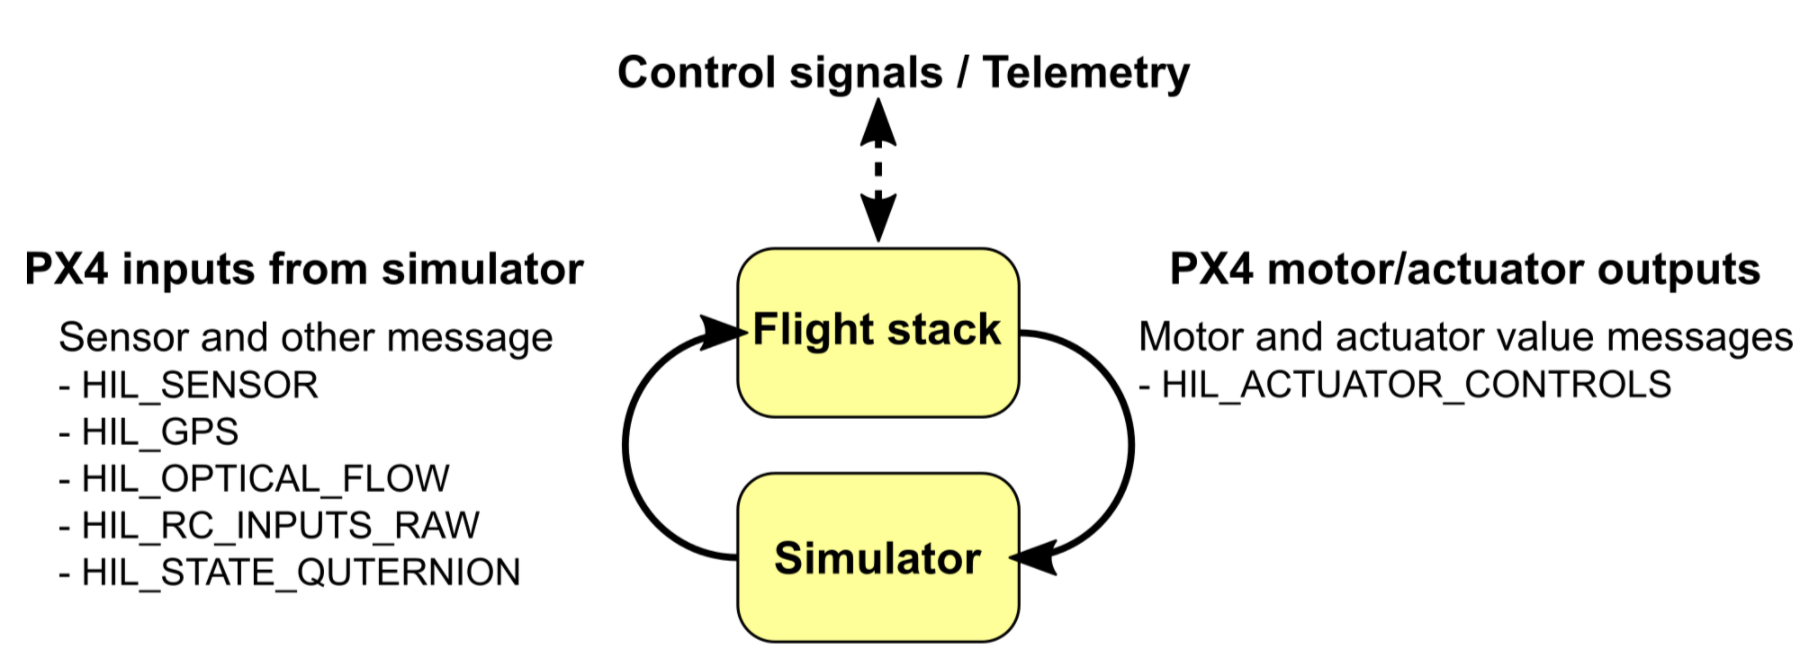
\includegraphics[scale=0.29]{obrazky/SIM1}
  \end{center}
  \caption[Tok zpráv mezi simulátorem a PX4]{Tok zpráv mezi simulátorem a PX4 \cite{SIM}.}
  \label{fig:SIM1}
\end{figure}

\section{SITL simulační prostředí}

\textit{\acl{SITL}} simulace umožňuje rychlé a \uv{levné} ladění robotických misí, protože pro simulaci \acs{SITL} se nevyužívá žádný specializovaný hardware, ale jenom počítač s nainstalovaným simulačním prostředím.

Obrázek \ref{fig:SIM2} zobrazuje typické prostředí simulace SITL v PX4 pro kterýkoliv z podporovaných simulátorů. Simulátor a PX4 firmawe mohou spolu komunikovat pomocí MAVLink \acs{API}. Pro přímou interakci s PX4 se využívá komunikace přes \textit{Micro-RTPS bridge}, kde se komunikují přímo uORB zprávy.

Různé části simulačního prostředí spolu komunikují pomocí \acs{UDP} (\acl{UDP}) a mohou být spuštěny na stejném počítači, nebo jiném počítači ve stejné síti. Pomocí sériové komunikace je možné připojit joystick, gamepad nebo RC soupravu pro ruční ovládání simulovaného dronu přes QGroundControl.

\begin{figure}[!ht]
  \begin{center}
    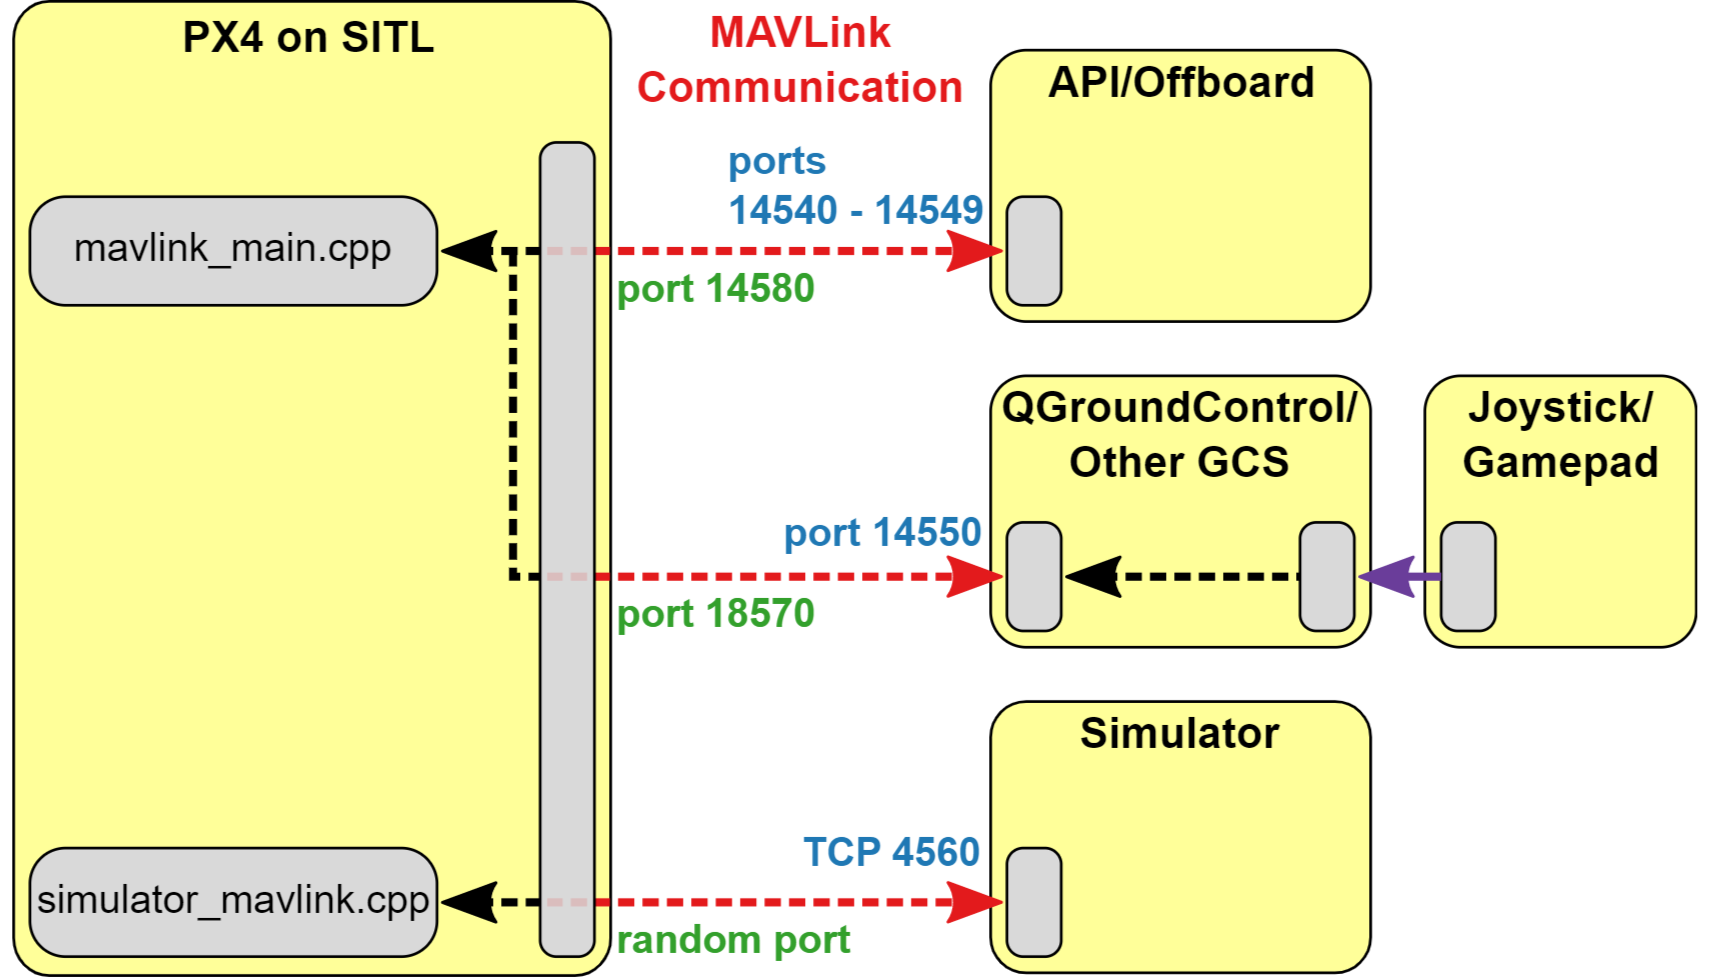
\includegraphics[scale=0.3]{obrazky/SIM2}
  \end{center}
  \caption[Diagram komunikace mezi PX4 a simulátorem]{Diagram komunikace mezi PX4 a simulátorem \cite{SIM}.}
  \label{fig:SIM2}
\end{figure}

\subsection{Seznam podporovaných simulátorů}

Následující simulátory jsou podporovány systémem PX4:

\begin{itemize}
    \item Gazebo
    \item FlightGear
    \item JSBSim
    \item jMAVSim
    \item AirSim
    \item Ignition Gazebo
\end{itemize}

\subsection{Gazebo}

Simulátor Gazebo je vysoce doporučen pro PX4 simulaci.

Gazebo je dobře navržený a otestovaný simulátor, umožňující rychlé testování algoritmů, návrh robotů a trénování systémů s umělou inteligencí v realistických scénářích. Nabízí možnost přesně a efektivně simulovat populace robotů ve složitých vnitřních i venkovních prostředích. Gazebo se běžně používá pro práci s ROS (ROS 2). \cite{GAZ}

Podporovaná vozidla \acs{SITL} simulace PX4 v simulátoru Gazebo jsou:

\begin{itemize}
    \item dron
    \item delta \acs{VTOL} (\acl{VTOL})
    \item letadlo
    \item rover
    \item ponorka
\end{itemize}

\subsection{Ignition Gazebo}

Vývojový tím simulátoru Gazebo se v budoucnu zaměří na vývoj simulátoru Ignition, takže Gazebo 11 je poslední verze známého simulátoru Gazebo. Oba simulátory jsou kompatibilní ve formátu popisu prostředí (\uv{světa}) a některých pluginů. \cite{IGN}

Z důvodu, že simulační firmware PX4 je v této době lépe propojený se simulátorem Gazebo, tak v této práci budeme pracovat s simulátorem Gazebo 11.

Jediné vozidlo, které je podporované \acs{SITL} simulací PX4 v simulátoru Ignition je dron.

\section{Instalace virtuálního prostředí}

Pro vývoj a simulaci bezpilotních misí v prostředí PX4 a ROS 2 je nutné nainstalovat jednotlivé komponenty vývojového prostředí:

\begin{itemize}
    \item PX4 simulační firmware
    \item Gazebo simulátor
    \item ROS 2 Foxy
    \item PX4 - ROS 2 \textit{bridge} (komunikační most mezi PX4 firmware a ROS 2)\\
\end{itemize}

V následujících podkapitolách si popíšeme instalaci jednotlivých částí. Návod je určený pro linuxovou distribuci Ubuntu 20.04 \textit{Focal Fossa}.

\subsection{Instalace PX4 simulačního prostředí}

Prvním krokem je instalace PX4 prostředí. Při reální misi (nebo \acs{HITL} simulaci) bude PX4 firmware spuštěný přímo na řídící jednotce Pixhawk. Při \acs{SITL} simulaci je nutné PX4 letový kód nainstalovat na počítač. Doporučená platforma pro PX4 prostředí je Ubuntu, ale je možné ho spustit na Windows 10 nebo na Mac OS.

Samotná instalace prostředí PX4 je jednoduchá a skládá se z 2 kroků. \cite{INSTALL1}

\begin{lstlisting}[language=bash]
# 1. Stáhnout zdrojový kód PX4:
$ git clone https://github.com/PX4/PX4-Autopilot.git --recursive
 
# 2. Spustit script ubuntu.sh bez argumentů
# pro instalaci všech závislostí
$ bash ./PX4-Autopilot/Tools/setup/ubuntu.sh
\end{lstlisting}

Script \texttt{ubuntu.sh} nastaví vývojové prostředí PX4, dále nainstaluje simulátory Gazebo a jMavSim a sadu nástrojů \textit{NuttX}\footnote{NuttX je \acs{RTOS} (\acl{RTOS}) pro provoz PX4 na řídící jednotce Pixhawk. Je to open source (BSD licence), lehký, výkonný a velmi stabilní operační systém. \cite{PX4main}}/\textit{Pixhawk}

\subsection{Instalace ROS 2 Foxy}

Instalace ROS 2 je dobře popsaná na dokumentačních stránkách \cite{ROS2INSTALL}. Po úspěšné instalaci ROS 2 Foxy je nutné doinstalovat několik závislostí:

\begin{lstlisting}[language=bash]
# 1. Instalační proces ROS 2 by měl nainstalovat 
# nástroje pro sestavení colcon, ale v případě, 
# že se tak nestane, můžete nástroje nainstalovat ručně:
$ sudo apt install python3-colcon-common-extensions
 
# 2. Eigen3 se používá v knihovně transformací:
$ sudo apt install ros-foxy-eigen3-cmake-module
 
# 3. Závislosti Pythonu musí být také nainstalovány:
$ sudo pip3 install -U empy pyros-genmsg setuptools
\end{lstlisting}

\subsection{Nastavení ROS 2 prostředí}

Pro vytvoření ROS 2 pracovního prostoru (\textit{workspace}) podporujícího simulaci v PX4 je nutné stáhnout dva ROS 2 balíčky. \cite{ROS2BRIDGE}

Na stáhnutí a sestavení obou balíčků můžeme použít tyto příkazy:

\begin{lstlisting}[language=bash]
# Naklonování obou balíčků:
$ mkdir -p ~/px4_ros_com_ros2/src
$ git clone https://github.com/PX4/px4_ros_com.git \
  ~/px4_ros_com_ros2/src/px4_ros_com
$ git clone https://github.com/PX4/px4_msgs.git \
  ~/px4_ros_com_ros2/src/px4_msgs
  
# Balíček px4_ros_com obsahuje scripty na sestavení workspace:
$ cd ~/px4_ros_com_ros2/src/px4_ros_com/scripts
$ source build_ros2_workspace.bash
\end{lstlisting}

\subsubsection{Balíček \texttt{px4\_msgs}}

V balíčku \texttt{px4\_msgs} je nadefinovaných víc jak 200 uORB zpráv pro komunikaci mezi ROS 2 \textit{node} a PX4 firmware.

\subsubsection{Balíček \texttt{px4\_ros\_com}}

Balíček \texttt{px4\_ros\_com} generuje přepojení mezi ROS 2 a PX4 firmware pomocí Fast RTPS (\acs{DDS}). V tomto balíčku je možné vytvářet ROS 2 misi pro autonomní řízení dronu.

\subsection{PX4 - ROS 2 bridge}

Jak je popsáno v kapitole \ref{sec:komunikace} \nameref{sec:komunikace}, pro komunikaci mezi ROS 2 \textit{node} a PX4 slouží \textit{eProsima Fast DDS}, který umožňuje výměnu zpráv uORB mezi PX4 a ROS 2.\\

Pro nastavení PX4 - ROS 2 \textit{bridge} potřebujeme nainstalovat následující balíčky:

\begin{itemize}
    \item Java JDK (Open source JDK 11)
    \item Gradle
    \item Fast-RTPS-Gen
\end{itemize}

\subsubsection{Java JDK a Gradle}

Java JDK a Gradle jsou nutné závislosti pro správnou funkci Fast-RTPS-Gen. Pro instalaci je možné použít návod zveřejněný zde: 

\href{https://linuxize.com/post/how-to-install-gradle-on-ubuntu-20-04/}{https://linuxize.com/post/how-to-install-gradle-on-ubuntu-20-04/} \cite{GRADLE}.

\subsubsection{Fast RTPS Gen}

Fast-RTPS-Gen je nástroj pro generování \acs{IDL} (\acl{IDL}) kódu pro Fast RTPS (\acs{DDS}).

Fast-RTPS-Gen je možné nainstalovat pomocí následujícího příkazu \cite{DDSGEN}:

\begin{lstlisting}[language=bash]
git clone --recursive https://github.com/eProsima/Fast-DDS-Gen.git \
    -b v1.0.4 ~/Fast-RTPS-Gen \
    && cd ~/Fast-RTPS-Gen \
    && gradle assemble \
    && sudo env "PATH=$PATH" gradle install
\end{lstlisting}

\acs{RTPS} agent se na palubním počítači spouští pomocí příkazu:

\begin{lstlisting}[language=bash]
$ source ~/px4_ros_com_ros2/install/setup.bash
$ micrortps_agent -t UDP
\end{lstlisting}

\section{ROS 2 misie}

Jedna možnost pro vytvoření autonomní mise v systému PX4 je pomocí programu QGroundControl, jak je popsáno v kapitole \ref{subs:planovani} \nameref{subs:planovani}. Zde je možné vytvořit jednoduché mise na průzkum prostředí, skenování koridoru, skenování konstrukcí a obecnou misi pomocí \textit{waypoints}. Celá mise musí být naplánovaná před startem, takže dron nemůže pohotově reagovat na různé situace, které nastanou v průběhu letu. 

Další možnost je vytvoření bezpilotní robotické mise v nadřazeném palubním počítači pomocí ROS 2 \textit{node}, který úkoluje řídící jednotku dronu. Tato možnost je vhodná pro složité mise, kde není před startem známá celá trajektorie letu a řídící algoritmus v palubním počítači ji dopočítává na základě čtení ze snímačů a kamer, nebo na základě povelů z pozemní stanice.

Pro tento případ jsme vytvořili ROS 2 \textit{node} (v C++), který komunikuje s PX4 firmware přes Fast RTPS. Zdrojový kód je zveřejněný na platformě GitHub \cite{GIT}.

Pro ovládání dronu z palubního počítače musí mít dron aktivovaný \textit{offboard flight mode} (mimopalubní letový režim).

\subsection{Offboard flight mode}

\textit{Offboard flight mode} se využívá vždy, když je dron řízený z jiného zdroje, než z Pixhawk řídící jednotky (PX4 firmware) například z palubního počítače. 

V \textit{offboard} letovém režimu se dronu posílají hlavě zprávy pro let na definovanou pozici (absolutní nebo relativní) a let určitým azimutem a rychlostí. Je vhodné, aby se pro kritické operace jako jsou vzlet, přistání, návrat na startovací pozici (\textit{Return to Launch}) využívali odpovídající letecké režimy.

Aby zůstal \textit{offboard} letový režim aktivní, palubní počítač musí posílat zprávu o aktivitě módu (\texttt{OffboardControlMode message}) s frekvencí > 2 Hz. V případě poruchy pablubního počítače, nebo nedostatečné rychlosti posílání zpráv se \textit{offboard} letový režim vypne a bude aktivovaný \textit{land} letový režim, takže dron přistane na daném místě. \cite{OFFBOADR}

\subsection{Výsledky simulace}

Pomocí ROS 2 \textit{node} se nám podařilo posílat zprávy do simulovaného PX4 firmware a tím ovládat dron v \textit{offboard} letovém režimu. Na obrázku \ref{fig:SIM3} v levém horním rohu je zobrazené, že dron je v režimu \textit{offboard flight mode}. Obrázek \ref{fig:SIM4} zobrazuje simulační prostředí Gazebo 11 které poskytuje fyzikální model \uv{světa} a graficky zobrazuje aktuální stav objektů v robotické misi.

\begin{figure}[!ht]
  \begin{center}
    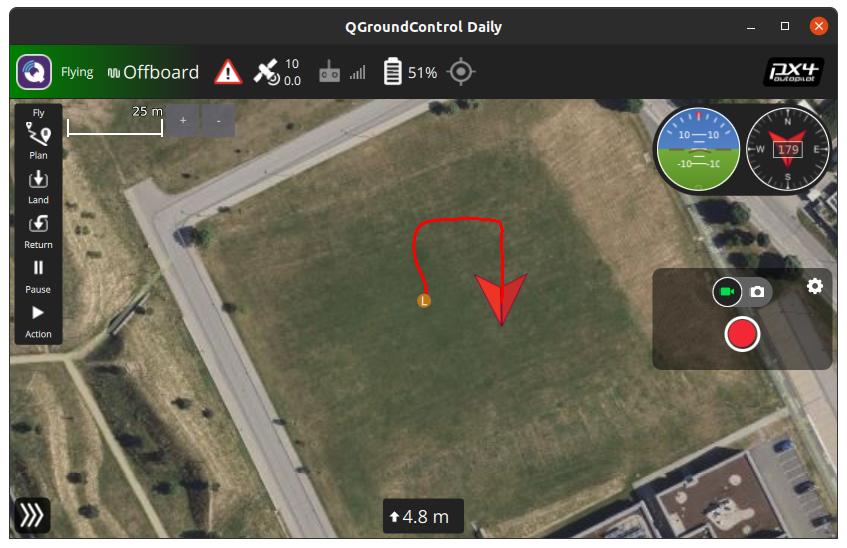
\includegraphics[scale=0.43]{obrazky/SIM3}
  \end{center}
  \caption[Software QGroundControl s dronem v \textit{offboard flight mode}]{Software QGroundControl s dronem v \textit{offboard flight mode}.}
  \label{fig:SIM3}
\end{figure}

\begin{figure}[!ht]
  \begin{center}
    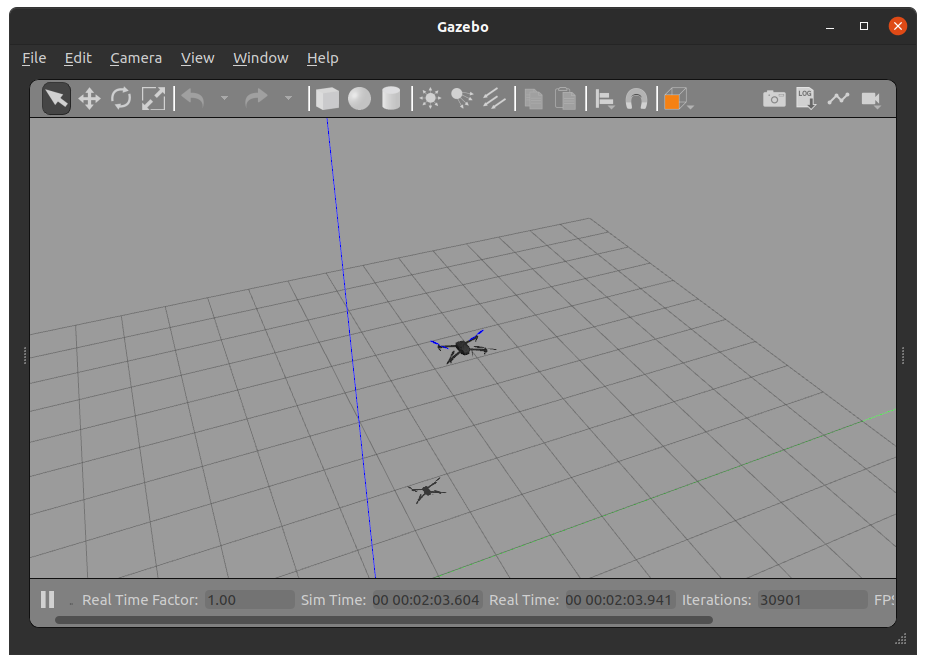
\includegraphics[scale=0.4]{obrazky/SIM4}
  \end{center}
  \caption[Bezpilotní mise v simulátoru Gazebo]{Bezpilotní mise v simulátoru Gazebo.}
  \label{fig:SIM4}
\end{figure}
\chapter{Implementace robotických misí}

Jedna možnost pro vytvoření autonomní mise v systému PX4 je pomocí programu QGroundControl, jak je popsáno v kapitole \ref{subs:planovani} \nameref{subs:planovani}. V tomto software je možné vytvořit jednoduché mise na průzkum prostředí, skenování koridoru, skenování konstrukcí a obecnou misi pomocí \textit{waypoints}. Celá mise musí být naplánovaná před startem, takže dron nemůže pohotově reagovat na různé situace, které nastanou v průběhu letu. 

Další možnost je vytvoření bezpilotní robotické mise v nadřazeném palubním počítači pomocí ROS 2 \textit{node}, který úkoluje řídící jednotku dronu. Tato možnost je vhodná pro složité mise, kde není před startem známá celá trajektorie letu a řídící algoritmus v palubním počítači ji dopočítává na základě čtení ze snímačů a kamer, nebo na základě povelů z pozemní stanice.

Pro tento případ jsme vytvořili několik ROS 2 uzlů (v C++), které komunikjí s PX4 firmware pomocí Fast RTPS, nebo pomocí MAVLink protokolu. Zdrojový kód je zveřejněný na platformě GitHub \cite{GIT}.

Pro ovládání dronu z palubního počítače musí mít dron aktivovaný \textit{offboard flight mode} (mimopalubní letový režim).

\section{Offboard flight mode}

\textit{Offboard flight mode} se využívá vždy, když je dron řízený z jiného zdroje, než z Pixhawk řídící jednotky (PX4 firmware), například z palubního počítače. 

V \textit{offboard} letovém režimu se dronu posílají hlavě zprávy pro let na definovanou pozici (absolutní nebo relativní), let určitým azimutem a rychlostí, nebo zprávy definující zrychlení dronu ve všech osách. Je vhodné, aby se pro kritické operace jako jsou vzlet, přistání, návrat na startovací pozici (\textit{Return to Launch}) využívali odpovídající letecké režimy řídící jednotky Pixhawk.

Aby zůstal \textit{offboard} letový režim aktivní, palubní počítač musí posílat zprávy o aktivitě módu (\texttt{OffboardControlMode message}) s frekvencí > 2 Hz.

V případě poruchy palubního počítače, nebo nedostatečné rychlosti posílání zpráv se \textit{offboard} letový režim vypne a bude aktivovaný předem bezpečný, definovaný letový režim, například \textit{land} letový režim, takže dron přistane na daném místě. \cite{PX4docs}

\section{Struktura robotické mise}

Jedním z cílů práce je navrhnout a implementovat ukázkovou robotickou misi pro autonomní létání dronů. V této kapitole se budeme zabývat námi implementovaným řešením robotické mise.

\subsection{Základní funkce dronu}

Vytvořili jsme základní třídu  v \texttt{C++} pro komunikaci s dronem pomocí protokolu MAVLink, která implementuje nezbytné funkce k řízení dronu. Při vytváření nové robotické mise se tato základní třída jednoduše zdědí a programátor se již nemusí zabývat implementací \textit{publisherů} a \textit{subscriberů} a může se soustředit na programování složitějších algoritmů robotické mise.

Dron je možné povelovat pomocí následujících funkcí, které jsou implementované v základní třídě:

\subsubsection{Funkce \texttt{arm}}

Funkce \texttt{arm} slouží k přepnutí dronu do \textit{arm} stavu, v kterém jsou motory aktivní a dron je schopen letu. Mimo tohoto stavu není možné dron ovládat. 

\subsubsection{Funkce \texttt{disarm}}

Funkce \texttt{disarm} přepíná dron do neaktivního (bezpečného) stavu, kdy není možné spustit motory dronu.

\subsubsection{Funkce \texttt{setFlightMode}}

Funkce \texttt{setFlightMode} mění letové režimy dronu. Víc o letových režimech je popsáno v kapitole \ref{sec:letRez} \nameref{sec:letRez}.

\subsubsection{Funkce \texttt{pullParam}}

Pro změnu vnitřních parametrů PX4 přez ROS 2 je nutné, aby spuštěný Mavros \textit{node} měl informaci o všech aktivních parametrech PX4. Funkce \texttt{pullParam} vyžádá všechny parametry z PX4.

\subsubsection{Funkce \texttt{preFlightCheck}}

Funkce \texttt{preFlightCheck} nastaví parametry PX4, které jsou nezbytné pro robotickou misi, jako jsou výška vzletu, horizontální rychlost, povolení \textit{offboard} módu a chování dronu po výpadku \textit{offboard módu}. Dále tato funkce zkontroluje, jestli proběhla korektní geolokace (GPS \textit{fix}).

\subsubsection{Funkce \texttt{publish\_traj\_setp\_position}}

Funkce \texttt{publish\_traj\_setp\_position} posílá do dronu \textit{setpoint} pro \textit{offboard} mód s relativní pozicí dronu vůči startovacímu místu. Když je dron přepnutý do \textit{offboard} módu a posíláme dronu setpointy s relativní pozicí, tak musí být tato funkce volána s frekvencí > 2 Hz.

\subsubsection{Funkce \texttt{publish\_traj\_setp\_speed}}

Funkce \texttt{publish\_traj\_setp\_speed} posílá do dronu příkazy pro let určitou lineární rychlostí v 3 osách a úhlovou rychlostí v 1 ose (\textit{yaw}). Při povelování dronu pomocí rychlostí vynecháváme poziční regulátor v firmware PX4, takže si ho musíme implementovat sami. Tato funkce musí být volána s frekvencí > 2 Hz, aby systém PX4 nevyhodnotil výpadek \textit{offboard} módu a neukončil misi předčasně.

\subsubsection{Funkce \texttt{publish\_traj\_setp\_geo}}

Funkce \texttt{publish\_traj\_setp\_geo} posílá dronu globální poziční \textit{setpoint} v souřadnicovém systému WGS 84. Pro setrvání v \textit{offboard} módu musí být tato funkce volána s frekvencí > 2 Hz.

\subsubsection{Funkce \texttt{isGlSetpReached}}

Funkce \texttt{isGlSetpReached} je pomocná funkce, která zjišťuje, zda dron v \textit{offboard} módu doletěl na nastavenou globální souřadnici.\\

Výše zmíněné funkce komunikují s dronem pomocí Mavros uzlu přes ROS 2 \textit{publishery}, \textit{subscribery} a \textit{clienty} (\textit{services}). Komunikace pomocí ROS 2 \textit{services} je výhodná pro kritické údaje kvůli tomu, že po odeslání požadavku z ROS 2 uzlu (například na změnu letového režimu, nebo nastavení vnitřních parametrů PX4) dostaneme od PX4 systému asynchronní odpověď, že požadavek byl zpracován.

Tabulka \ref{tab:pubsub} zobrazuje a popisuje všechny ROS 2 \textit{publishery}, \textit{subscribery} a \textit{clienty} (\textit{services}), které využívá základní třída dronu.

\begin{table}[!ht]
\catcode`\-=12
  \caption[Přehled využitých objektů typu publisher, subscriber a client]{Přehled využitých objektů typu \textit{publisher}, \textit{subscriber} a \textit{client} v základní třídě dronu.}
  \label{tab:pubsub}
  \begin{center}
  	  \def\arraystretch{1.1}
	  \begin{tabular}{|c|c|c|}
	    \hline
	    \rowcolor{light-gray}
	    Objekt & ROS 2 zpráva & Popis  \\
	    \hline
        \multirow{4}{*}{\rotatebox{90}{Subscriber}} & \texttt{mavros\_msgs::msg::State} & Stav řídící jednotky \\
        \cline{2-3}
        & \texttt{mavros\_msgs::msg::Altitude} & Nadmořská výška \\ 
        \cline{2-3}
        & \texttt{sensor\_msgs::msg::NavSatFix} & Pozice podle WGS 84 \\
        \cline{2-3}
        & \texttt{geometry\_msgs::msg::PoseStamped} & Relativní pozice \\ 
        \hline
        \multirow{3}{*}{\rotatebox{90}{Publisher}} & \texttt{geometry\_msgs::msg::PoseStamped} & Setpoint pro lokální pozici \\
        \cline{2-3}
        & \texttt{geometry\_msgs::msg::TwistStamped} & Setpoint pro  nastavení rychlostí\\ 
        \cline{2-3}
        & \texttt{geographic\_msgs::msg::GeoPoseStamped} & Setpoint pro globální pozici \\
        \hline
        \multirow{3}{*}{\rotatebox{90}{Client}} & \texttt{mavros\_msgs::srv::CommandBool} & Nastavení \texttt{arm} nebo \texttt{disarm} \\
        \cline{2-3}
        & \texttt{mavros\_msgs::srv::SetMode} & Nastavení letových režimů \\ 
        \cline{2-3}
        & \texttt{mavros\_msgs::srv::ParamSetV2} & Nastavení parametrů PX4 \\
        \cline{2-3}
        & \texttt{mavros\_msgs::srv::ParamPull} & Vyžádání všech parametrů \\
        \hline
	  \end{tabular}
  \end{center}
\end{table}

\subsection{Struktura řídícího algoritmu}

Všechny námi implementované robotické mise mají stejnou základní strukturu algoritmu. Pro řízení mise je využitý jeden hlavní stavový automat, který ovládá všechny úkony od vzletu až po ukončení mise.

Kromě vzletu, kde je použitý \textit{take off} letový režim je v celé robotické misi využíván \textit{offboard} letový režim, v kterém dron vykonává všechny další úkony. Podle typu robotické mise řídící systém posílá dronu v \textit{offboard} letovém režimu lokální nebo globální poziční waypointy, nebo rychlostní setpointy.

\subsection{Stavový automat pro řízení mise}

Na obrázku \ref{fig:MISE2} jsou zobrazeny kroky základního stavového automatu pro řízení námi implementovaných misí.

V následující části jsou popsány stavy a podmínky přechodů v stavovém automatu pro řízení mise:

\begin{figure}[!ht]
  \begin{center}
    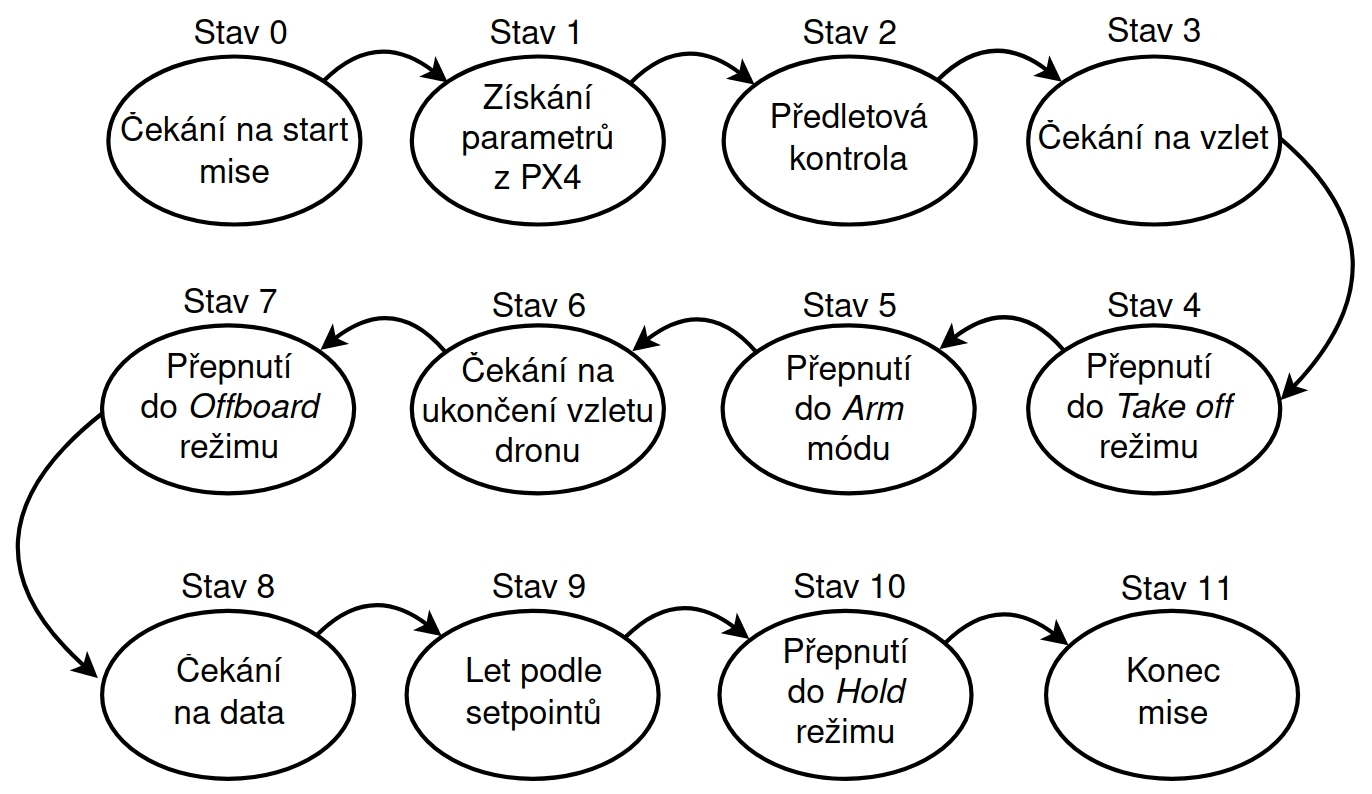
\includegraphics[scale=0.32]{obrazky/MISEAUTOMAT}
  \end{center}
  \caption[Stavový automat řídící robotickou misi]{Stavový automat řídící robotickou misi.}
  \label{fig:MISE2}
\end{figure}

\subsubsection{Stav 0: Čekání na start mise}

Dron je na zemi ve vypnutém stavu.

\noindent\textbf{Podmínka přechodu:} Uběhne uživatelem stanovený čas.

\subsubsection{Stav 1: Získání parametrů z PX4}

Dron vyžádá aktivní parametry ze systému PX4 kvůli tomu, aby bylo možné měnit parametry pomocí komunikačního uzlu Mavros.

\noindent\textbf{Podmínka přechodu:} Komunikační uzel Mavros pošle nadřazenému uzlu, který řídí misi informaci, že systém PX4 poskytl všechny aktivní parametry.

\subsubsection{Stav 2: Předletová kontrola}

V tomto kroku dron vykoná nezbytné kontroly letové způsobilosti jako je kontrola korektní geolokace (GPS \textit{fix}) a nastaví důležité parametry robotické mise jako je výška vzletu, horizontální rychlost, povolení \textit{offboard módu} a chování dronu po výpadku \textit{offboard} módu.

\noindent\textbf{Podmínka přechodu:} Systém PX4 odešle informaci, že všechny parametry byly změněny správně a GPS na dronu je aktivní.

\subsubsection{Stav 3: Čekání na vzlet}

Dron je na zemi ve vypnutém stavu.

\noindent\textbf{Podmínka přechodu:} Uběhne uživatelem stanovený čas.

\subsubsection{Stav 4: Přepnutí dronu do \textit{take off} letového režimu}

Nadřazený systém pošle požadavek pro změnu letového režimu na \textit{take off} letový režim.

\noindent\textbf{Podmínka přechodu:} Systém PX4 pošle odpověď, že letový režim dronu byl úspěšně změněný.

\subsubsection{Stav 5: Přepnutí dronu do \textit{arm} módu}

Nadřazený systém pošle požadavek pro změnu letového režimu.

\noindent\textbf{Podmínka přechodu:} Systém PX4 pošle odpověď, že mód dronu byl úspěšně změněný na \textit{arm}.

\subsubsection{Stav 6: Čekání na ukončení vzletu dronu}

Dron vykonává sekvenci úkonů pro vzlet.

\noindent\textbf{Podmínka přechodu:} Nadřazený systém detekuje změnu letového režimu na \textit{hold} letový režim z důvodu ukončení vzletu.

\subsubsection{Stav 7: Přepnutí dronu do \textit{offboard} letového režimu}

Nadřazený systém pošle požadavek pro změnu letového režimu na \textit{offboard} letový režim.

\noindent\textbf{Podmínka přechodu:} Systém PX4 pošle odpověď, že letový režim dronu byl úspěšně změněný.

\subsubsection{Stav 8: Čekání na data}

Dron se vznáší v \textit{offboard} letovém režimu na místě, kde byla ukončená vzletová sekvence. Tento stav je aktivní jenom v misích, kde jsou data pro let dronu generována a vysílána jiným ROS 2 uzlem, například v misi pro sledování dynamického objektu.

\noindent\textbf{Podmínka přechodu:} ROS 2 uzel pro řízení mise přijme první paket dat.

\subsubsection{Stav 9: Let podle setpointů}

Dron v \textit{offboard} letovém režimu vykonává jednotlivé úkony robotické mise. Nadřazený ROS 2 uzel pro řízení mise posílá dronu buď poziční waypointy (lokální nebo globální), nebo řídí přímo lineární rychlosti v osách \textit{X}, \textit{Y}, \textit{Z} a rychlost rotace kolem osy \textit{Z}.

\noindent\textbf{Podmínka přechodu:} Nadřazený uzel pro řízení mise již nepřímá data pro let dronu (po určitou dobu definovanou uživatelem), nebo dron vykoná všechny úkony robotické mise.

\subsubsection{Stav 10: Přepnutí do \textit{hold} režimu}

Dron se v tomto stavu vznáší v \textit{offboard} letovém režimu na místě, kde ukončil poslední úkon robotické mise. V této fázi je nutný zásah pilota kvůli tomu, že nechceme, aby dron zahájil přistávací manévr bez vědomí a povolení pilota.

\noindent\textbf{Podmínka přechodu:} Pilot dronu převezme řízení dronu.

\subsubsection{Stav 11: Konec mise}

Pilot dronu přistává, nebo zahajuje další autonomní misi.


\chapter{Výsledky simulace}

V této kapitole jsou popsány námi implementované mise s bezpilotními letadly ve virtuálním prostředí. 

Simulace pozůstávala z fyziky reálného světa, kterou nám poskytoval robotický simulátor Gazebo. Dále byl simulován firmware PX4, který běží v řídící jednotce dronu a nakonec ROS 2 uzel, který posílá povely systému PX4 a tím řídí samotný průběh robotické mise.

\section{Gzebo svět}

Díky spolupráci se studentem bc. Milošem Cihlářem jsme získali třírozměrnou reprezentaci území mezi Vědeckotechnickým parkem prof. Lista a sportovním areálem CESA v okolí Fakulty elektrotechniky a komunikačních technologií VUT v Brně. 

Kvůli tomu, že je tento model možné importovat do robotického simulátoru Gazebo, jsou všechny zpracované simulované mise zasazeny do reálného území v blízkosti naší školy, jak je zobrazeno na obrázcích \ref{fig:SIM3QGC}, \ref{fig:SIM3GAZ}, \ref{fig:SIM3MULQG} a \ref{fig:SIM3MULGAZ}.

\section{Let podle waypointů}

Funkčnost simulace jsme demonstrovali na robotické misi jejímž cílem byl let dronu po waypointech. Pro tento účel jsme implementovali dvě alternativy, a to řízení dronu na lokální, a globální waypointy.

V obou případech jsou data o trajektorii letu známá před misí. Tyto data se načítají z \texttt{.yaml} souboru jako ROS 2 parametry, takže je možné je měnit bez kompilace celého zdrojového kódu mise. 

\subsection{Let podle lokálních waypointů}

Zprávy typu \texttt{geometry\_msgs::msg::PoseStamped} jsou z nadřazeného uzlu publikovány do ROS 2 témy (\textit{topic}) \texttt{/mavros/setpoint\_position/local} s frekvencí 10 Hz (pro aktivitu \textit{offboard} letového režimu musí být zprávy posílány s frekvencí > 2 Hz).

\subsection{Let podle globálních waypointů}

Zprávy typu \texttt{geographic\_msgs::msg::GeoPoseStamped} jsou z nadřazeného uzlu publikovány do ROS 2 témy (\textit{topic}) \texttt{/mavros/setpoint\_position/global} s frekvencí 10 Hz.

\section{Let podle setpointů rychlosti}

Další robotická mise, na které jsme otestovali funkčnost simulace je založená na řízení dronu podle lineární rychlosti v osách X, Y, Z a rychlosti rotace kolem osy Z. 

Řízení tohoto typu je vhodné v případě, že regulační smyčka v PX4 (obrázek \ref{fig:PX4controller}) nepostačuje našim požadavkům na regulaci a tudíž musíme implementovat vlastní, komplexnější řídící strukturu. Obrázek \ref{fig:PX4controller} zobrazuje, že při řízení dronu pomocí setpointů rychlosti vynecháme PX4 poziční regulátor\footnote{Poziční regulátor V PX4 je složený z P složky a saturace} z řídící struktury.

Další možností, kterou jsme neimplementovali je řízení dronu pomocí setpointů lineárního zrychlení v osách \textit{X}, \textit{Y} a \textit{Z}. Tímto krokem by jsme vynechali taky rychlostní regulátor\footnote{Rychlostní regulátor V PX4 je složený z PID složky a saturace} z řídící struktury PX4 a měli by jsme volnou ruku při implementaci komplexnějších řídících struktur.

\begin{figure}[!ht]
  \begin{center}
    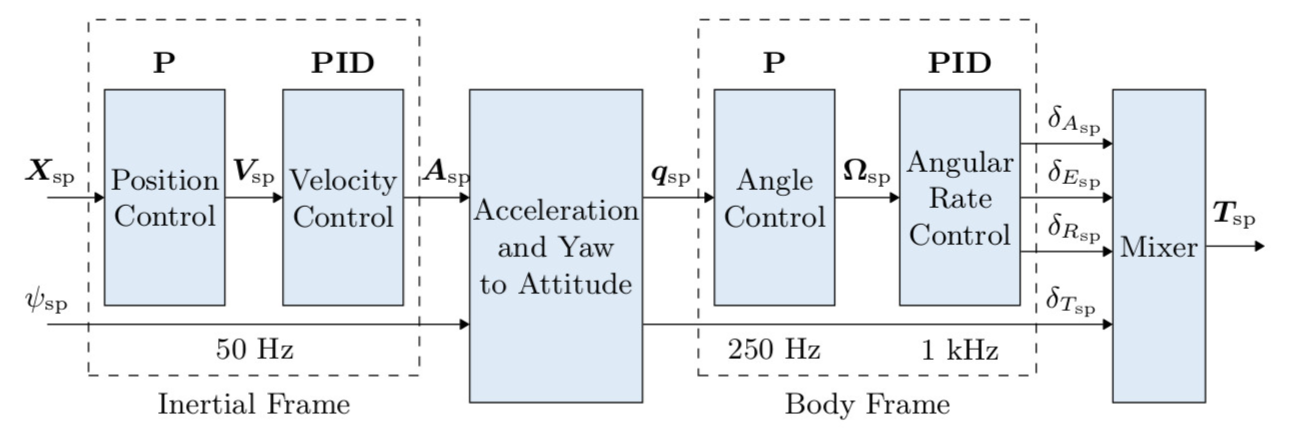
\includegraphics[scale=0.44]{obrazky/PX4CONTROLLER}
  \end{center}
  \caption[Řídící struktura systému PX4]{Řídící struktura systému PX4. \cite{PX4docs}}
  \label{fig:PX4controller}
\end{figure}

Zprávy typu \texttt{geometry\_msgs::msg::TwistStamped} jsou z nadřazeného uzlu publikovány do ROS 2 témy (\textit{topic}) \texttt{/mavros/setpoint\_velocity/cmd\_vel} s frekvencí 10 Hz.

\section{Mise pro sledování dynamického objektu}

Funkčnost simulace jsme také demonstrovali na složitější robotické misi jejímž cílem bylo sledování dynamického objektu. 

Pro tuto úlohu jsme využili data z měření radiace pomocí všesměrového radiačního detektoru, který byl umístěný na pozemním robotu. Robot pomocí částicového filtru (\textit{particle filter}) estimoval pozici radioaktivního zářiče a na základě této estimace se k zdroju radiace přibližoval. Celá mise byla prováděna v okolí Fakulty elektrotechniky a komunikačních technologií VUT v Brně.

Data z měření jsme měli k dispozici jako \texttt{rosbag} soubor\footnote{Rosbag soubor slouží na zálohu dat v podobě ROS 2 témat (\textit{topic})}, který obsahuje zprávy typu \texttt{geographic\_msgs::msg::GeoPoseStamped} a publiku je do ROS 2 tématu \texttt{/estimated\_source\_location}. Tyto zprávy obsahují globální souřadnice estimovaného zdroje radiace podle standardu WGS 84. Dron se v průběhu celé mise pohybuje v konstantní výšce, která de definovatelná uživatelem pomocí ROS 2 parametru.

Na obrázku \ref{fig:SIM3QGC} je zobrazený software QGroundControl s trajektorii mise pro sledování dynamického objektu. V levém horním rohu můžeme vidět, že dron je přepnutý do \textit{offboard} letového režimu. Jak je možné vidět na obrázku, simulovaná mise byla prováděna taky v okolí Fakulty elektrotechniky a komunikačních technologií VUT v Brně. Počáteční souřadnice mise byla 49.22812907° severní šířky, 16.57222321° východní délky, v nadmořské výšce 283 metrů.

\begin{figure}[!ht]
  \begin{center}
    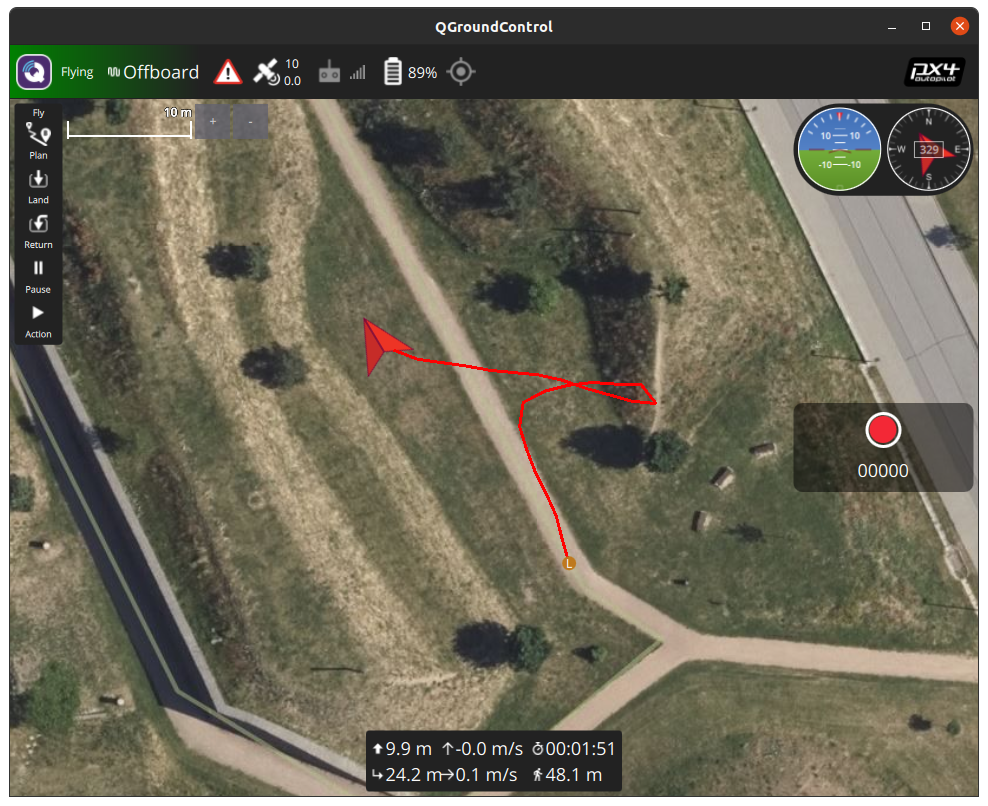
\includegraphics[scale=0.40]{obrazky/MISESL1}
  \end{center}
  \caption[Mise pro sledování dynamického objektu v software QGroundControl]{Mise pro sledování dynamického objektu v software QGroundControl.}
  \label{fig:SIM3QGC}
\end{figure}

Obrázek \ref{fig:SIM3GAZ} zobrazuje vzlet dronu v průběhu simulované mise pro sledování dynamického objektu v robotickém simulačním prostředí Gazebo 11.

\begin{figure}[!ht]
  \begin{center}
    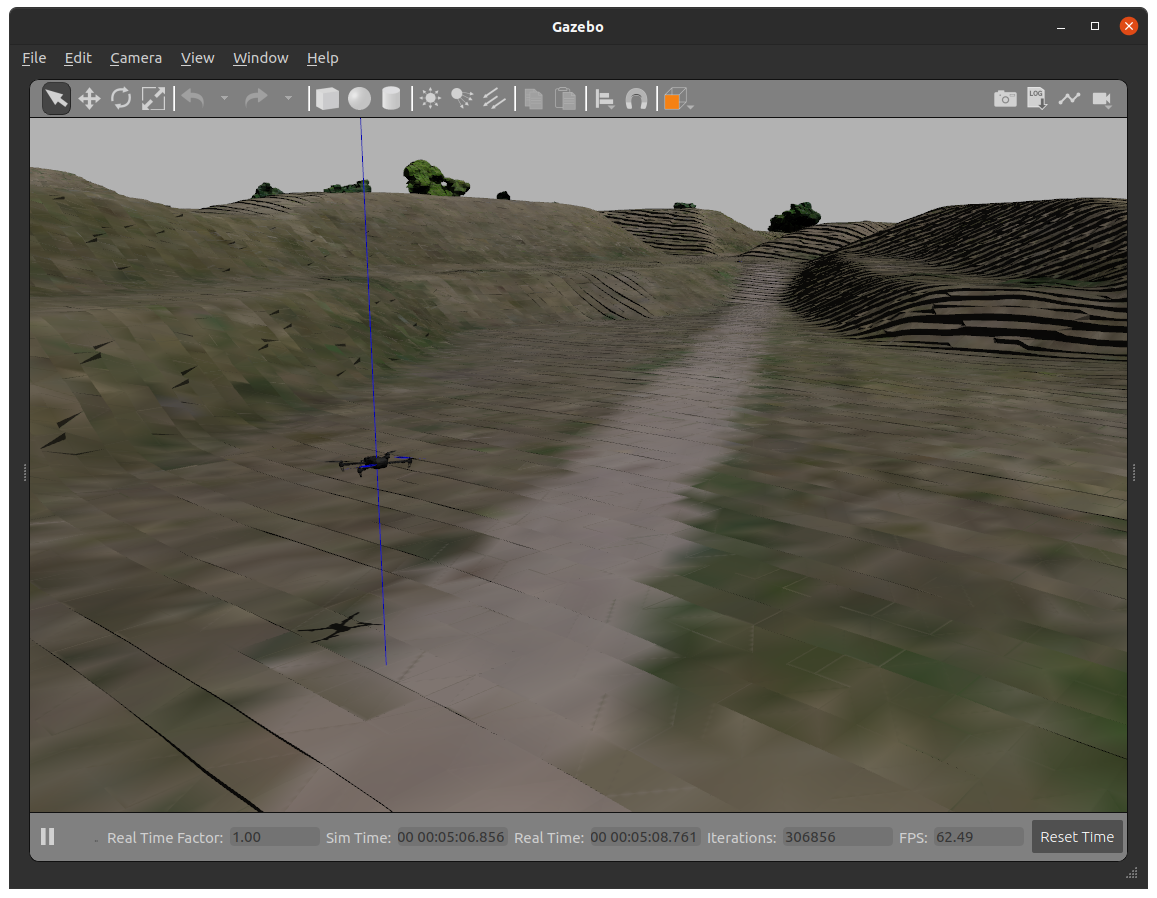
\includegraphics[scale=0.35]{obrazky/GAZSIMPLE.png}
  \end{center}
  \caption[Mise pro sledování dynamického objektu v simulačním software Gazebo 11]{Mise pro sledování dynamického objektu v simulačním software Gazebo 11.}
  \label{fig:SIM3GAZ}
\end{figure}


\section{Simulace misí s více drony}

Dalším z cílů práce bylo zobecnit navržené řešení tak, aby bylo možné simulovat mise s více bezpilotními letadly najednou. Z důvodu modularity systému ROS (ROS 2) nebyla tato úloha složitá. Pomocí \texttt{.launch} souboru jsme nadefinovali všechny ROS 2 uzly, které se mají spustit. Ke každému uzlu je nadefinovaný ROS 2 \texttt{namespace} tak, aby každý uzel pro řízení mise komunikoval se správným Mavros uzlem a tím taky se správným simulovaným dronem.

\subsection{Mise pro sledování dynamického objektu s více drony}

Obrázek \ref{fig:SIM3MULQG} 

DOKONCIT

\begin{figure}[!ht]
  \begin{center}
    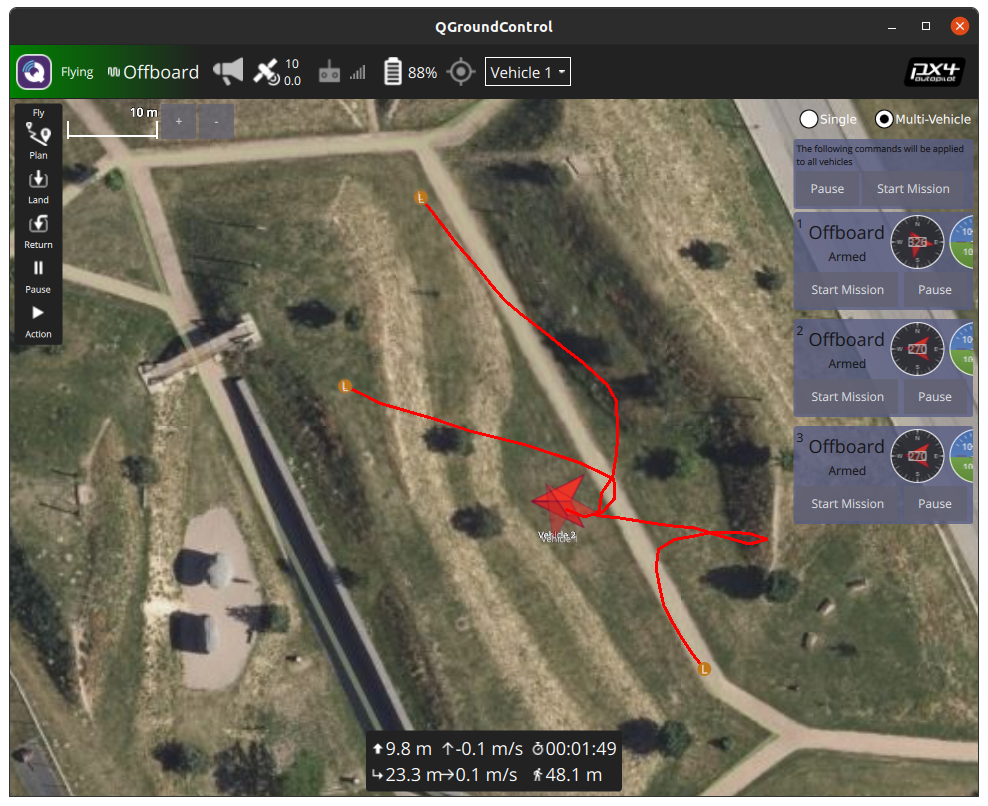
\includegraphics[scale=0.41]{obrazky/QGMULTIPLE.png}
  \end{center}
  \caption[Mise pro sledování dynamického objektu s více drony v software QGroundControl]{Mise pro sledování dynamického objektu s více drony v software QGroundControl.}
  \label{fig:SIM3MULQG}
\end{figure}

Obrázek \ref{fig:SIM3MULGAZ}

DOKONCIT

\begin{figure}[!ht]
  \begin{center}
    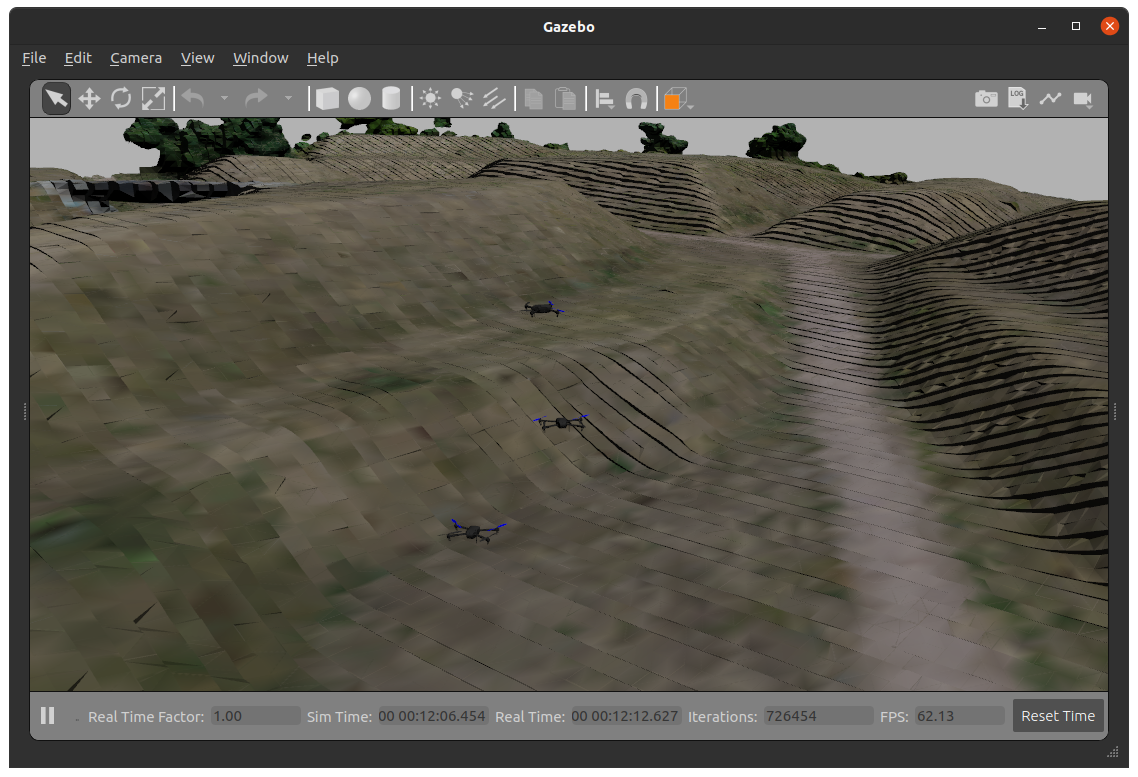
\includegraphics[scale=0.38]{obrazky/GAZMULTIPLE.png}
  \end{center}
  \caption[Mise pro sledování dynamického objektu s více drony v software Gazebo 11]{Mise pro sledování dynamického objektu s více drony v software Gazebo 11.}
  \label{fig:SIM3MULGAZ}
\end{figure}



\chapter*{Závěr}
\phantomsection
\addcontentsline{toc}{chapter}{Závěr}

ZÁVER DOKONČIŤ

Tato semestrální práce se zabývala problematikou simulace misí bezpilotních letadel ve virtuálním prostředí ROS2/Gazebo. V první kapitole je popsána topologie dronu z pohledu řídícího systému. Zaobírá se jak řídící jednotkou pro nízkoúrovňové řízení dronu, tak palubním počítačem pro řízení složitých autonomních misí.

V další kapitole je popsán firmware pro řídící jednotku Pixhawk. Kapitola pojednává o architektuře firmware PX4 a o možnostech propojení a komunikace s ostatními periferiemi. Nedílnou součástí ekosystému PX4 je software QGroundControl pro vzdálenou kontrolu letu, plánování různých typů bezpilotních misí a nastavení dronu.

Důležitou částí práce je popis komunikace mezi ROS 2 a PX4 firmware přes Fast RTPS (\acs{DDS}) bridge. Práce rozebírá samotný \acs{DDS} (\acl{DDS}) middleware a jeho komunikační protokol \acs{RTPS} (\acl{RTPS}) pro kritické aplikace, základní vlastnosti \acs{DDS} a hlavně propojení mezi ROS 2 a \acs{DDS} komunikačním middleware.

Poslední kapitola popisuje simulaci ve virtuálním ekosystému PX4 - Gazebo - ROS 2. Shrnuje instalaci všech závislostí a postup sestavení simulačního prostředí (\textit{workspace}). Kapitola se zabývá tvořením a plánováním autonomní robotické mise, která je realizována pomocí ROS 2 balíčku a její testováním v simulačním prostředí. Cílem jednoduché autonomní mise je ovládat dron v tzv. \textit{offboard} módu pomocí ROS 2 balíčku. Podařilo se nám odsimulovat bezpilotní misi složenou z vzletu dronu, přeletu přes několik relativních souřadnic a následného přistání.



%%% Vložení souboru 'text/literatura' se seznamem zdrojů
% Pro sazbu seznamu literatury použijte jednu z následujících možností

%%%%%%%%%%%%%%%%%%%%%%%%%%%%%%%%%%%%%%%%%%%%%%%%%%%%%%%%%%%%%%%%%%%%%%%%%
%1) Seznam citací definovaný přímo pomocí prostředí literatura / thebibliography

\begin{thebibliography}{99}

    \bibitem{MRS}
MRS UAV System - open source platform for UAV research. \textit{Multi-robot Systems Group} [online]. Praha: Multi-robot Systems Group, c2022 [cit. 2022-01-01]. Dostupné z: \href{http://mrs.felk.cvut.cz/}{http://mrs.felk.cvut.cz/}

    \bibitem{PIX1}
The open standards for drone hardware. \textit{Pixhawk} [online]. San Francisco: Dronecode, 2018 [cit. 2022-01-01]. Dostupné z: \href{https://pixhawk.org/}{https://pixhawk.org/}

    \bibitem{PIX2}
Pixhawk 4. \textit{PX4} [online]. San Francisco: Dronecode, 2021 [cit. 2022-01-01]. Dostupné z: \href{https://docs.px4.io/master/en/flight\_controller/pixhawk4.html}{https://docs.px4.io/master/en/flight\_controller/pixhawk4.html}

	\bibitem{BSDlicense}
The 3-Clause BSD License: BSD-3-Clause. \textit{Open Source Initiative} [online]. West Hollywood: Open Source Initiative, 2014 [cit. 2021-11-17]. Dostupné z: \href{https://opensource.org/licenses/BSD-3-Clause}{https://opensource.org/licenses/BSD-3-Clause}

    \bibitem{PX4main}
PX4 Architectural Overview. \textit{PX4 Autopilot User Guide} [online]. San Francisco: Dronecode, 2021 [cit. 2021-12-19]. Dostupné z: \href{https://docs.px4.io/master/en/concept/architecture.html}{https://docs.px4.io/master/en/concept/architecture.html}

    \bibitem{PX4main2}
PX4 System Architecture. \textit{PX4 Autopilot User Guide} [online]. San Francisco: Dronecode, 2021 [cit. 2021-12-20]. Dostupné z: \href{https://docs.px4.io/master/en/concept/px4\_systems\_architecture.html}{https://docs.px4.io/master/en/concept/px4\_systems\_architecture.html}

	\bibitem{QGround}
QGroundControl. \textit{QGroundControl} [online]. San Francisco: Dronecode, 2019 [cit. 2021-11-24]. Dostupné z: \href{http://qgroundcontrol.com/}{http://qgroundcontrol.com/}

    \bibitem{QGround2}
QGroundControl User Guide. \textit{QGroundControl docs} [online]. San Francisco: Dronecode, 2021 [cit. 2021-12-21]. Dostupné z: \href{https://docs.qgroundcontrol.com/master/en/PlanView/Pattern.html}{https://docs.qgroundcontrol.com/master/en/PlanView/Pattern.html}

    \bibitem{ROS2DDS3}
ROS 2 middleware interface: Mapping between DDS and ROS concepts. \textit{ROS 2 Design} [online]. California: Open Source Robotics Foundation, 2017 [cit. 2021-12-21]. Dostupné z: \href{https://design.ros2.org/articles/ros\_middleware\_interface.html}{https://design.ros2.org/articles/ros\_middleware\_interface.html}

    \bibitem{UORB1}
UORB Messaging. \textit{PX4 Autopilot User Guide} [online]. San Francisco: Dronecode, 2021 [cit. 2021-12-21]. Dostupné z: \href{https://docs.px4.io/master/en/middleware/uorb.html}{https://docs.px4.io/master/en/middleware/uorb.html}

    \bibitem{UORBlist}
UORB Message Reference. \textit{PX4 Autopilot User Guide} [online]. San Francisco: Dronecode, 2021 [cit. 2021-12-24]. Dostupné z: \href{https://docs.px4.io/master/en/msg\_docs/}{https://docs.px4.io/master/en/msg\_docs/}

    \bibitem{UORB2}
RTPS/DDS Interface: PX4-Fast RTPS(DDS) Bridge. \textit{PX4 Autopilot User Guide} [online]. San Francisco: Dronecode, 2021 [cit. 2021-12-21]. Dostupné z: \href{https://docs.px4.io/master/en/middleware/micrortps.html}{https://docs.px4.io/master/en/middleware/micrortps.html}

    \bibitem{CDR}
EProsima Fast Buffers. \textit{EProsima the middleware experts} [online]. Madrid: eProsima, 2014 [cit. 2021-12-23]. Dostupné z: \href{https://www.eprosima.com/docs/fast-buffers/0.3.0/html/index.html}{https://www.eprosima.com/docs/fast-buffers/0.3.0/html/index.html}

    \bibitem{DDS_Standard}
The Real-time Publish-Subscribe Protocol (RTPS) DDS Interoperability Wire Protocol Specification. \textit{Object Management Group} [online]. Milford: OMG, c2021 [cit. 2021-11-25]. Dostupné z: \href{https://www.omg.org/spec/DDSI-RTPS/2.3}{https://www.omg.org/spec/DDSI-RTPS/2.3}
	
	\bibitem{DDS_Def}
Data Distribution Service (DDS). \textit{Object Management Group} [online]. Milford: OMG, 2018 [cit. 2021-11-25]. Dostupné z: \href{https://www.omg.org/omg-dds-portal/}{https://www.omg.org/omg-dds-portal/}

    \bibitem{DDS_Main}
What is DDS? \textit{DDS Foundation: Join DDS Foundation} [online]. Milford: DDS Foundation, c1997-2021 [cit. 2021-11-25]. Dostupné z: \href{https://www.dds-foundation.org/what-is-dds-3/}{https://www.dds-foundation.org/what-is-dds-3/}

    \bibitem{DDS_usage}
Why choose DDS?: Industry standards build on top of DDS. \textit{DDS Foundation: Join DDS Foundation} [online]. Milford: DDS Foundation, c1997-2021 [cit. 2021-11-25]. Dostupné z: \href{https://www.dds-foundation.org/why-choose-dds/}{https://www.dds-foundation.org/why-choose-dds/}

    \bibitem{DDS_PubSub}
Introduction to Publish/Subscribe. \textit{Real-Time Innovations: RTI | Inteligent, distributed and real world systems} [online]. Sunnyvale: RTI, c2020 [cit. 2021-11-28]. Dostupné z: \href{https://community.rti.com/static/documentation/connext-dds/6.0.1/doc/manuals/connext\_dds/getting\_started/cpp11/intro\_pubsub\_cpp.html}{https://community.rti.com/static/documentation/connext-dds/6.0.1/doc/manuals/connext\_cpp11/intro\_pubsub\_cpp.html}

    \bibitem{Eprosima}
RTPS Introduction: What is RTPS? \textit{EProsima: The Middleware experts} [online]. Madrid: eProsima, c2013-2021 [cit. 2021-11-29]. Dostupné z: \href{https://www.eprosima.com/index.php/resources-all/whitepapers/rtps}{https://www.eprosima.com/index.php/resources-all/whitepapers/rtps}

    \bibitem{ROS2DDS}
ROS on DDS: Technical Credibility of DDS. \textit{ROS 2 Design} [online]. California: Open Source Robotics Foundation, c2021 [cit. 2021-11-29]. Dostupné z: \href{https://design.ros2.org/articles/ros\_on\_dds.html}{https://design.ros2.org/articles/ros\_on\_dds.html}


    \bibitem{ROS2DDS2}
About different ROS 2 DDS/RTPS vendors: Supported RMW implementations. \textit{ROS 2 Documentation: Foxy} [online]. California: Open Robotics, c2021 [cit. 2021-12-09]. Dostupné z: \href{https://docs.ros.org/en/foxy/Concepts/About-Different-Middleware-Vendors.html}{https://docs.ros.org/en/foxy/Concepts/About-Different-Middleware-Vendors.html}

    \bibitem{SIM}
Simulation. \textit{PX4 Autopilot User Guide} [online]. San Francisco: Dronecode, 2021 [cit. 2021-12-28]. Dostupné z: \href{https://docs.px4.io/master/en/simulation/}{https://docs.px4.io/master/en/simulation/}

    \bibitem{GAZ}
\textit{Gazebo} [online]. California: Open Source Robotics Foundation, c2014 [cit. 2021-12-30]. Dostupné z: \href{http://gazebosim.org/}{http://gazebosim.org/}

    \bibitem{IGN}
THACKSTON, Allison. Ignition vs Gazebo. \textit{Allison Thackston} [online]. San Francisco: Thackston, c2014-2021 [cit. 2021-12-31]. Dostupné z: \href{https://www.allisonthackston.com/articles/ignition-vs-gazebo.html}{https://www.allisonthackston.com/articles/ignition-vs-gazebo.html}



% \bibitem{sr02/2009}
% 		VUT v~Brně:
%     \emph{Úprava, odevzdávání a zveřejňování vysokoškolských kva\-li\-fi\-kač\-ních prací na VUT v~Brně}\/ [online].
% 		Směrnice rektora č.\,2/2009.
% 		Brno: 2009, po\-sled\-ní aktualizace 24.\,3.\,2009 [cit.\,23.\,10.\,2015].
%     Dostupné z~URL:\\
%     <\url{https://www.vutbr.cz/uredni-deska/vnitrni-predpisy-a-dokumenty/smernice-rektora-f34920/}>.

% \bibitem{CSN_ISO_690-2011}
%     \emph{ČSN ISO 690 (01 0197) Informace a dokumentace -- Pravidla pro bibliografické odkazy a citace informačních zdrojů.}
%     40 stran. Praha: Český normalizační institut, 2011.

% \bibitem{CSN_ISO_7144-1997}
%     \emph{ČSN ISO 7144 (010161) Dokumentace -- Formální úprava disertací a podobných dokumentů.}
%     24 stran. Praha: Český normalizační institut, 1997.

% \bibitem{CSN_ISO_31-11}
%     \emph{ČSN ISO 31-11 Veličiny a jednotky -- část 11: Matematické znaky a značky používané ve fyzikálních vědách a v~technice.}
%     Praha: Český normalizační institut, 1999.

% \bibitem{BiernatovaSkupa2011:CSNISO690komentar}
%     BIERNÁTOVÁ, O., SKŮPA, J.:
%     \emph{Bibliografické odkazy a citace dokumentů dle ČSN ISO 690 (01 0197) platné od 1.\,dubna 2011}\/ [online].
%     2011, poslední aktualizace 2.\,9.\,2011 [cit. 19.\,10.\,2011].
%     Dostupné z~URL:
%     \(<\)\url{http://www.citace.com/CSN-ISO-690.pdf}\(>\)
% %    \(<\)\href{http://www.boldis.cz/citace/citace.html}{http://www.boldis.cz/citace/citace.html}\(>\).

% \bibitem{pravidla}
%     \emph{Pravidla českého pravopisu}.
%     Zpracoval kolektiv autorů. 1.\ vydání.
%     Olomouc: FIN PUB\-LISH\-ING, 1998. 575 s. ISBN 80-86002-40-3.

% \bibitem{Walter1999}
% 	WALTER, G.\,G.; SHEN, X.
% 	\emph{Wavelets and Other Orthogonal Systems}.
% 	2. vyd. Boca Raton: Chapman\,\&\,Hall/CRC, 2000. 392~s. ISBN 1-58488-227-1

% \bibitem{Svacina1999IEEE}
% 	SVAČINA, J.
% 	Dispersion Characteristics of Multilayered Slotlines -- a Simple Approach.
% 	\emph{IEEE Transactions on Microwave Theory and Techniques},
% 	1999, vol.\,47, no.\,9, s.\,1826--1829. ISSN 0018-9480.

% \bibitem{RajmicSysel2002}
%     RAJMIC, P.; SYSEL, P.
%     Wavelet Spectrum Thresholding Rules.
%     In \emph{Proceedings of the International Conference Research in Telecommunication Technology},
%     Žilina: Žilina University, 2002. s.\,60--63. ISBN 80-7100-991-1.

\end{thebibliography}


%%%%%%%%%%%%%%%%%%%%%%%%%%%%%%%%%%%%%%%%%%%%%%%%%%%%%%%%%%%%%%%%%%%%%%%%%
%%2) Seznam citací pomocí BibTeXu
%% Při použití je nutné v TeXnicCenter ve výstupním profilu aktivovat spouštění BibTeXu po překladu.
%% Definice stylu seznamu
%\bibliographystyle{unsrturl}
%% Pro českou sazbu lze použít styl czechiso.bst ze stránek
%% http://www.fit.vutbr.cz/~martinek/latex/czechiso.tar.gz
%%\bibliographystyle{czechiso}
%% Vložení souboru se seznamem citací
%\bibliography{text/literatura}
%
%% Následující příkaz je pouze pro ukázku sazby literatury při použití BibTeXu.
%% Způsobí citaci všech zdrojů v souboru literatura.bib, i když nejsou citovány v textu.
%\nocite{*}

%%% Vložení souboru 'text/zkratky' se seznam použitých symbolů, veličin a zkratek
\cleardoublepage
\chapter*{\listofabbrevname}
\phantomsection
\addcontentsline{toc}{chapter}{\listofabbrevname}

\begin{acronym}[KolikMista]

	\acro{IMU}
		[IMU]
		{Inertial Measurement Unit}
		
	\acro{SITL}
		[SITL]
		{Software In The Loop}
		
	\acro{HITL}
		[HITL]
		{Hardware In The Loop}
		
	\acro{CDR}
		[CDR]
		{Common Data Representation}
		
	\acro{API}
		[API]
		{Application programming interface}

    \acro{DDS}
		[DDS\textsuperscript \textregistered ]
		{Data-Distribution Service\textsuperscript \textregistered}
		
    \acro{RTPS}
		[RTPS]
		{Real Time Publish Subscribe protocol}
		
	\acro{DDSI}
	    [DDSI-RTPS\textsuperscript{\texttrademark} ]
	    {DDS Interoperability Wire Protocol\textsuperscript{\texttrademark}}
		
    \acro{QoS}
		[QoS]
		{Quality of Service}
		
	\acro{UDP}
		[UDP]
		{User datagram protocol}
		
	\acro{VTOL}
		[VTOL]
		{Vertical Take-Off and Landing}
		
	\acro{RTOS}
		[RTOS]
		{Real-Time Operating System}
		
	\acro{IDL}
		[IDL]
		{Interactive Data Language}
		
\end{acronym}


%%% Začátek příloh
\appendix

%%% Vysázení seznamu příloh
% (vynechejte, pokud máte dvě nebo méně příloh)
% \listofappendices

%%% Vložení souboru 'text/prilohy' s přílohami
% Obvykle je přítomen alespoň popis co najdeme na přiloženém médiu
\chapter{Přílohy}

\chapter{Obsah elektronické přílohy}
Elektronická příloha je často nedílnou součástí semestrální nebo závěrečné práce.
Vkládá se do informačního systému VUT v~Brně ve vhodném formátu (ZIP, PDF\,\dots).

Nezapomeňte uvést, co čtenář v~této příloze najde.
Je vhodné okomentovat obsah každého adresáře, specifikovat, který soubor obsahuje důležitá nastavení, který soubor je určen ke spuštění, uvést nastavení kompilátoru atd.
Také je dobře napsat, v~jaké verzi software byl kód testován (např.\ Matlab 2018b).
Pokud bylo cílem práce vytvořit hardwarové zařízení,
musí elektronická příloha obsahovat veškeré podklady pro výrobu (např.\ soubory s~návrhem DPS v~Eagle).

Pokud je souborů hodně a jsou organizovány ve více složkách, je možné pro výpis adresářové struktury použít balíček \href{https://www.ctan.org/pkg/dirtree}{\texttt{dirtree}}.

\bigskip

{\small
%
\dirtree{%.
.1 /\DTcomment{kořenový adresář přiloženého archivu}.
.2 logo\DTcomment{loga školy a fakulty}.
.3 BUT\_abbreviation\_color\_PANTONE\_EN.pdf.
.3 BUT\_color\_PANTONE\_EN.pdf.
.3 FEEC\_abbreviation\_color\_PANTONE\_EN.pdf.
.3 FEKT\_zkratka\_barevne\_PANTONE\_CZ.pdf.
.3 UTKO\_color\_PANTONE\_CZ.pdf.
.3 UTKO\_color\_PANTONE\_EN.pdf.
.3 VUT\_barevne\_PANTONE\_CZ.pdf.
.3 VUT\_symbol\_barevne\_PANTONE\_CZ.pdf.
.3 VUT\_zkratka\_barevne\_PANTONE\_CZ.pdf.
.2 obrazky\DTcomment{ostatní obrázky}.
.3 soucastky.png.
.3 spoje.png.
.3 ZlepseneWilsonovoZrcadloNPN.png.
.3 ZlepseneWilsonovoZrcadloPNP.png.
.2 pdf\DTcomment{pdf stránky generované informačním systémem}.
.3 student-desky.pdf.
.3 student-titulka.pdf.
.3 student-zadani.pdf.
.2 text\DTcomment{zdrojové textové soubory}.
.3 literatura.tex.
.3 prilohy.tex.
.3 reseni.tex.
.3 uvod.tex.
.3 vysledky.tex.
.3 zaver.tex.
.3 zkratky.tex.
%.2 navod-sablona\_FEKT.pdf\DTcomment{návod na používání šablony}.
.2 sablona-obhaj.tex\DTcomment{hlavní soubor pro sazbu prezentace k~obhajobě}.
%.2 readme.txt\DTcomment{soubor s~popisem obsahu CD}.
.2 sablona-prace.tex\DTcomment{hlavní soubor pro sazbu kvalifikační práce}.
.2 thesis.sty\DTcomment{balíček pro sazbu kvalifikačních prací}.
}
}


\end{document}
